% Foliensatz: "AFu-Kurs nach DJ4UF" von DK0TU, Amateurfunkgruppe der TU Berlin
% Lizenz: CC BY-NC-SA 3.0 de (http://creativecommons.org/licenses/by-nc-sa/3.0/de/)
% Autoren: Felix Baum DB4UM <baum@campus.tu-berlin.de>

\documentclass[aspectratio=169]{beamer}

\usepackage[ngerman]{babel} % deutsche Worttrennung etc.
\usepackage[utf8]{inputenc} % UTF8 Text

\usepackage[super, comma, numbers, square, sort]{natbib}

\usepackage{hyperref}       % Hyperref Package für bessere Referenzen (todo)
\hypersetup{
	colorlinks=false,       %   false: boxed links; true: colored links
    %linkcolor=white,       %   color of internal links (change box color with linkbordercolor)
    citecolor=red,          %   color of links to bibliography
    filecolor=white,        %   color of file links
    urlcolor=blue           %   color of external links
}

\usepackage{multirow}
\usepackage{wasysym}  % Math Symbols like \permil
%\usepackage{colortbl}
%\usepackage{subscript}
%\usepackage{caption}
%\usepackage{setspace}
%\usepackage{xcolor}        % benutze CodeListe

% Footnote
%\usepackage{hanging}
%
%\setbeamertemplate{footnote}{%
%  \hangpara{2em}{1}%
%  \makebox[2em][l]{\insertfootnotemark}\footnotesize\insertfootnotetext\par%
%}


%\usepackage{pgf}
%\usepackage{tikz}
%\usetikzlibrary{arrows,automata}
%\usetikzlibrary{positioning}
%
%\tikzset{
%    state/.style={
%           rectangle,
%           rounded corners,
%           draw=black, very thick,
%           minimum height=2em,
%           minimum width=2pt,
%           inner sep=2pt,
%           text centered,
%           },
%}

%\usepackage{listings}
%\lstset{basicstyle=\small, numberstyle=\tiny, extendedchars=true, numbers=left, numbersep=5pt}
%\lstset{showtabs=false, showspaces=false, showstringspaces=false}
%%\lstset{backgroundcolor=\color{white!75!lightgray}, , frame=single}
%%\lstset{backgroundcolor=\color{white}}
%%\lstset{backgroundcolor=none}
%\lstset{keywordstyle=\color{blue!50!gray},  identifierstyle=\color{black}}
%\lstset{commentstyle=\color{green!50!gray}, stringstyle=\color{red!50!gray}}
%\lstset{language=C, fontadjust=true, tabsize=2, breaklines=true}
%\lstset{backgroundcolor=\color{white!75!lightgray}, caption=\lstname, frame=single}
%\lstset{emphstyle=\color{black}\fbox}
%
%% Keine "Listing:"-Caption
%\captionsetup{labelformat=empty,labelsep=none}
%
%% für mathematische Umgebungen
%\usepackage{amsmath,amsfonts,amssymb}
%
%\lstdefinestyle{Bash}{
%language=Bash,
%frame=single,
%rulecolor=\color{black},
%backgroundcolor=\color{gray!50},
%keywordstyle=\color{black},
%identifierstyle=,
%commentstyle=\color{black},
%stringstyle=\color{magenta!65!white},
%showstringspaces=false,
%basicstyle=\footnotesize\ttfamily\color{black},
%numbers=none,
%breaklines=true,
%captionpos=b
%}

%\usepackage{listings}
%
%\lstdefinestyle{basic}{
%    captionpos=t,%
%    basicstyle=\footnotesize\ttfamily,%
%    numberstyle=\tiny,%
%    numbers=left,%
%    stepnumber=1,%
%    frame=single,%
%    showspaces=false,%
%    showstringspaces=false,%
%    showtabs=false,%
%    %
%    keywordstyle=\color{blue},%
%    identifierstyle=,%
%    commentstyle=\color{gray},%
%    stringstyle=\color{magenta}%
%}



% fließende Boxen haben keinen Abstand
%\fboxsep0mm

% inkludiere Creative Commons Helper
%%%%%%%%%%%%%%%%%%%%%%%%%%%%%%%%%%%%%%%%%%%%%%%%%%%%%%%%%%%%%%%%
%% ccBeamer 0.1, 2007-07-02                                   %%
%% Written by Sebastian Pipping <webmaster@hartwork.org>      %%
%% ---------------------------------------------------------- %%
%% Licensed under Creative Commons Attribution-ShareAlike 3.0 %%
%% http://creativecommons.org/licenses/by-sa/3.0/             %%
%%%%%%%%%%%%%%%%%%%%%%%%%%%%%%%%%%%%%%%%%%%%%%%%%%%%%%%%%%%%%%%%


%% Images
\newcommand{\CcImageBy}[1]{%
	
\includegraphics[scale=#1]{texdata/creative_commons/cc_by_30.pdf}%
}
\newcommand{\CcImageCc}[1]{%
	
\includegraphics[scale=#1]{texdata/creative_commons/cc_cc_30.pdf}%
}
\newcommand{\CcImageDevNations}[1]{%
	
\includegraphics[scale=#1]{texdata/creative_commons/cc_dev_nations_30.pdf}%
}
\newcommand{\CcImageNc}[1]{%
	
\includegraphics[scale=#1]{texdata/creative_commons/cc_nc_30.pdf}%
}
\newcommand{\CcImageNd}[1]{%
	
\includegraphics[scale=#1]{texdata/creative_commons/cc_nd_30.pdf}%
}
\newcommand{\CcImagePd}[1]{%
	
\includegraphics[scale=#1]{texdata/creative_commons/cc_pd_30.pdf}%
}
\newcommand{\CcImageSa}[1]{%
	
\includegraphics[scale=#1]{texdata/creative_commons/cc_sa_30.pdf}%
}
\newcommand{\CcImageSampling}[1]{%
	
\includegraphics[scale=#1]{texdata/creative_commons/cc_sampling_30.pdf}%
}
\newcommand{\CcImageSamplingPlus}[1]{%
	
\includegraphics[scale=#1]{texdata/creative_commons/cc_sampling_plus_30.pdf}%
}


%% Groups
\newcommand{\CcGroupBy}[2]{% zoom, gap
	\CcImageCc{#1}\hspace*{#2}\CcImageBy{#1}%
}
\newcommand{\CcGroupByNc}[2]{% zoom, gap
	\CcImageCc{#1}\hspace*{#2}\CcImageBy{#1}\hspace*{#2}\CcImageNc{#1}%
}
\newcommand{\CcGroupByNcNd}[2]{% zoom, gap
	\CcImageCc{#1}\hspace*{#2}\CcImageBy{#1}\hspace*{#2}\CcImageNc{#1}\hspace*{#2}\CcImageNd{#1}%
}
\newcommand{\CcGroupByNcSa}[2]{% zoom, gap
	\CcImageCc{#1}\hspace*{#2}\CcImageBy{#1}\hspace*{#2}\CcImageNc{#1}\hspace*{#2}\CcImageSa{#1}%
}
\newcommand{\CcGroupByNd}[2]{% zoom, gap
	\CcImageCc{#1}\hspace*{#2}\CcImageBy{#1}\hspace*{#2}\CcImageNd{#1}%
}
\newcommand{\CcGroupBySa}[2]{% zoom, gap
	\CcImageCc{#1}\hspace*{#2}\CcImageBy{#1}\hspace*{#2}\CcImageSa{#1}%
}
\newcommand{\CcGroupDevNations}[2]{% zoom, gap
	\CcImageCc{#1}\hspace*{#2}\CcImageDevNations{#1}%
}
\newcommand{\CcGroupNcSampling}[2]{% zoom, gap
	\CcImageCc{#1}\hspace*{#2}\CcImageNc{#1}\hspace*{#2}\CcImageSampling{#1}%
}
\newcommand{\CcGroupPd}[1]{% zoom
	\CcImagePd{#1}%
}
\newcommand{\CcGroupSampling}[1]{% zoom
	\CcImageSampling{#1}%
}
\newcommand{\CcGroupSamplingPlus}[1]{% zoom
	\CcImageSamplingPlus{#1}%
}


%% Text
\newcommand{\CcLongnameBy}{Attribution}
\newcommand{\CcLongnameByNc}{Attribution-NonCommercial}
\newcommand{\CcLongnameByNcNd}{Attribution-NoDerivs}
\newcommand{\CcLongnameByNcSa}{Attribution-NonCommercial-ShareAlike}
\newcommand{\CcLongnameByNd}{Attribution-NoDerivs}
\newcommand{\CcLongnameBySa}{Attribution-ShareAlike}

\newcommand{\CcNote}[1]{% longname
	This work is licensed under the \textit{Creative Commons #1 3.0 License}.%
}


% generelles Thema auswählen
\usetheme{Goettingen} %Berlin spart ohne Sidebar allerdings angenehm Platz
% AnnArbor | Antibes | Bergen | Berkeley | Berlin | Boadilla | boxes | CambridgeUS | Copenhagen | Darmstadt | default | Dresden | Frankfurt | Goettingen | Hannover | Ilmenau | JuanLesPins | Luebeck | Madrid | Malmoe | Marburg | Montpellier | PaloAlto | Pittsburgh | Rochester | Singapore | Szeged | Warsaw

% Farben wählen
\usecolortheme{beetle}
% beaver | beetle | crane | default | dolphin | dove | fly | lily | orchid | rose | seagull | seahorse | sidebartab | structure | whale | wolverine

% Setze alle Farben auf Grau und Weiß
%\definecolor{craneorange}{RGB}{64,64,64}
%\definecolor{craneblue}{RGB}{255,255,255}

% Schriftart wählen
\usefonttheme{default}
% default | professionalfonts | serif | structurebold | structureitalicserif | structuresmallcapsserif

% Innere Themen(Kopf-, Fuß-, Sidebar usw)
%\useinnertheme{default}
\useinnertheme{circles}
% default | inmargin | rectangles | rounded | circles

% Äußere Themen (Anordnung der inneren, grenzen der Folien etc.)
\useoutertheme{infolines}
% default | infolines | miniframes | shadow | sidebar | smoothbars | smoothtree | split | tree

% Deaktiviere Navigations-Symbole ({} -> leer)
\setbeamertemplate{navigation symbols}{}
%\setbeamertemplate{navigation symbols}{\large \ifnum \insertframenumber <10 0\fi\insertframenumber/\inserttotalframenumber\vspace*{0.2ex}}

% Zeige ein Hintergrundbild
\setbeamertemplate{background canvas}{
        \hspace*{-2.0cm}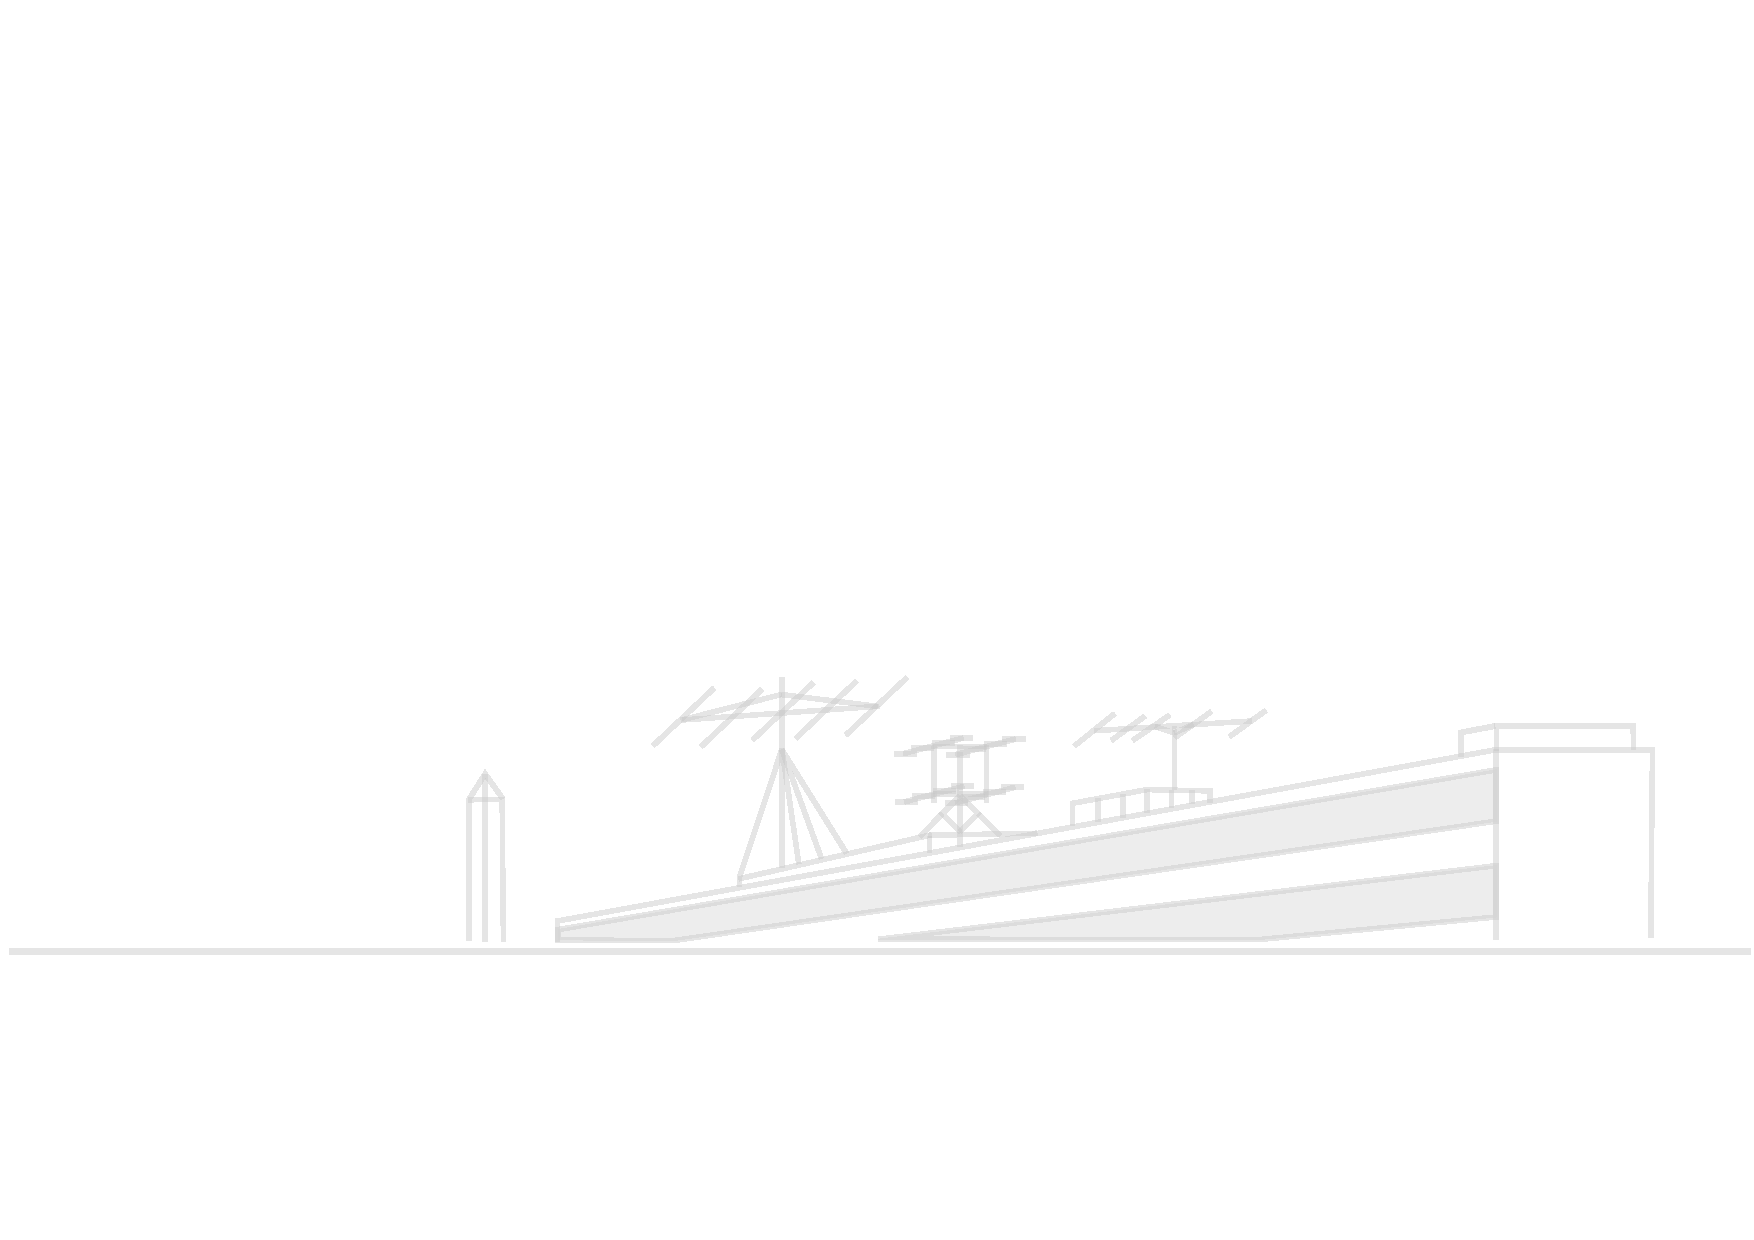
\includegraphics[width=17.8cm]{texdata/dk0tu_rooftop_background.pdf}
}

% Foliennummer einfügen
\setbeamertemplate{footline}[frame number]
%\setbeamertemplate{footline}{}

% Ändere das Zeichen vor jedem item
%\setbeamertemplate{itemize item}{\color{craneorange}$\blacktriangleright$}
%\setbeamertemplate{itemize subitem}{\color{craneorange}$\triangleright$}
%\setbeamertemplate{itemize subsubitem}{\color{craneorange}$\blacktriangleright$}

% Ändert die Blöcke 
\setbeamertemplate{blocks}[rounded][shadow=true]
% default | rounded [shadow=true|false]

%
% Eigene Kommandos
%

% Hack to get natbib and beamer working together. "The beamer user guide suggests
% that only the manual bibliography entry approach is supported"
% on some system it works out of the box, sometimes you need the hack :-(
% so check it --dl7bst
\ifdefined\newblock
    \relax
\else
    \newcommand{\newblock}{}
\fi

% \includedia command to generate png out of a dia file
% NEEDS installed dia and pdflatex option --shell-escape
\newcommand{\includedia}[1]{
    \immediate\write18{/usr/bin/dia #1.dia -e #1_diatmp.png -t png}
}

% RICHIG GROSSER FONT!
\newfont{\bigfont}{cmr10 at 144pt}
\newfont{\smallfont}{cmr10 at 8pt}

% Römische Ziffern
\makeatletter
\newcommand{\rmnum}[1]{\romannumeral #1}
\newcommand{\Rmnum}[1]{\expandafter\@slowromancap\romannumeral #1@}
\makeatother

% Schwarze Überschrift
%\setbeamercolor{frametitle}{fg=black}
%\setbeamercolor{title}{fg=black}

% Item- und Box-Farben
\definecolor{deepBlue}{HTML}{000066}
\setbeamercolor{itemize item}{fg=deepBlue}
\setbeamercolor{itemize subitem}{fg=deepBlue}
\setbeamercolor{description item}{fg=deepBlue}
\setbeamercolor{block title}{fg=deepBlue!100, bg=blue!15}
\setbeamercolor{block body}{fg=black, bg=blue!5}
\setbeamercolor{block title alerted}{fg=deepBlue, bg=red!75}
\setbeamercolor{block body alerted}{fg=black, bg=red!15}
\setbeamercolor*{block title example}{fg=blue!50, bg=blue!10}
\setbeamercolor*{block body example}{fg= blue, bg=blue!5}

%\setbeamercolor{section in head/foot}{parent=palette primary}
%\setbeamercolor{subsection in head/foot}{parent=palette secondary}
%\setbeamercolor{sidebar}{fg=darkblue,bg=yellow!90!orange}
%\setbeamercolor{title in sidebar}{fg=darkblue}
%\setbeamercolor{author in sidebar}{fg=darkblue}
%\setbeamercolor{section in sidebar}{fg=darkblue!10!black}
%\setbeamercolor{subsection in sidebar}{fg=darkblue!50!black}

% Titlepage Infos
\title{AFu-Kurs nach DJ4UF}
\author[DKØTU]{DKØTU\\ \footnotesize{Amateurfunkgruppe der TU Berlin}}
\institute[DKØTU]{\url{http://www.dk0tu.de} }

% PDF-Eigenschaften
\subject{DK0TU-Amateurfunkkurs nach DJ4UF}
\keywords{Amateurfunk Kurs HAM Radio Course CC-BY-NC-SA OpenSource TU Berlin DK0TU}

\subtitle{Technik A09: \\
  Antennentechnik  \\[2em]}
\date{Stand 01.06.2015}
 \begin{document}

\begin{frame}
    \titlepage
    \vfill
    \begin{center}
        \ccbyncsaeu\\
        {\tiny This work is licensed under the \em{Creative Commons Attribution-NonCommercial-ShareAlike 3.0 License}.}\\[0.5ex]
         \tiny Amateurfunkgruppe der Technische Universität Berlin (AfuTUB), DKØTU
         %\includegraphics[scale=0.5]{img/DK0TU_Logo.pdf}
    \end{center}
\end{frame}


\section*{Wiederholung}

\begin{frame}
  \frametitle{Antenne}
  \begin{center}
    \includegraphics[width=.6\textwidth]{e11/Traqueur_acquisition.JPG}
    \tiny \hyperlink{refs}{\cite{wm}}
  \end{center}
\end{frame}

\begin{frame}
  \frametitle{Strom und Spannungsverteilung}
  \begin{center}
    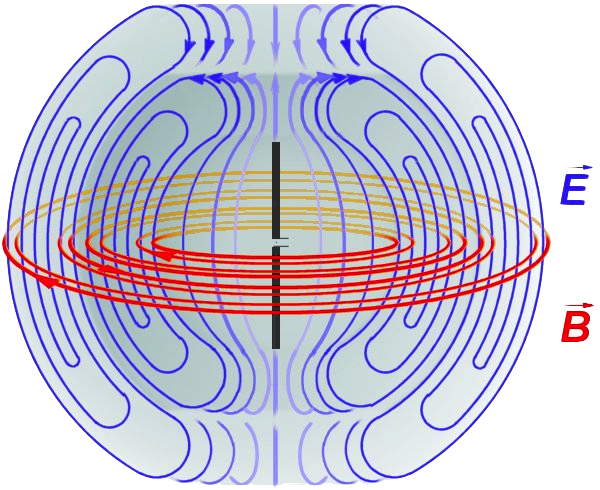
\includegraphics[width=0.8\textwidth]{a09/Felder_um_Dipol.png}
    \tiny \hyperlink{refs}{\cite{wm}} \\[1em] \large
  \end{center}
\end{frame}

\begin{frame}
  \frametitle{Stromverteilung Dipol}
  \begin{center}
    \Large Wie verteilen sich Strom und Spannung auf einem Dipol? \\ (Bäuche und Knoten)
  \end{center}
\end{frame}

\begin{frame}
  \frametitle{Strom und Spannungsverteilung}
  \begin{center}
    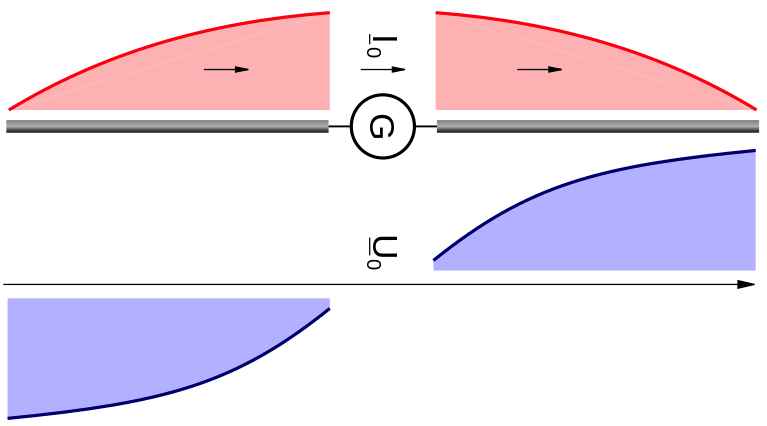
\includegraphics[width=0.8\textwidth]{a09/DipolUI.png}
    \tiny \hyperlink{refs}{\cite{wm}} \\[1em] \large
  \end{center}
\end{frame}

\begin{frame}
  \frametitle{Verschiedene Frequenzen}
  \begin{center}
    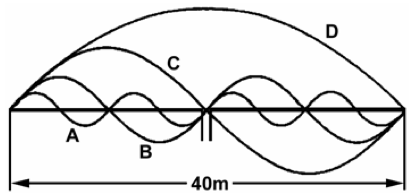
\includegraphics[width=0.8\textwidth]{a09/TH108.png} \\
    \tiny \hyperlink{refs}{\cite{bna}} TH108\\[1em] \large
    Die Wellen zeigen die Stromverteilung am Dipol. \\Welche Frequenz ist welcher Buchstabe?
  \end{center}
\end{frame}


\section*{Antennenimpedanz}

\begin{frame}
  \frametitle{Antennenimpedanz Dipol}
  \begin{center}
    \begin{itemize}
      \item Dipol hat je nach Höhe über dem Boden unterschiedliche Impedanz \\[1em]
      \item Lambda-Halbe Dipol hat eine Impedanz von ca 60 - 75 Ohm \\[1em]
      \item Beim Lambda-Halbe Dipol rein reeller Widerstand \\[1em]
      \item Welche Impedanz hat ein Lambda-Halbe-Dipol unterhalb und oberhalb seiner Grundfrequenz? \\[1em]
    \end{itemize}
  \end{center}
\end{frame}

\begin{frame}
  \frametitle{Komplexe Eingangsimpedanzen}
  \begin{center}
    \begin{itemize}
      \item Welche Impedanz hat ein Lambda-Halbe-Dipol unterhalb und oberhalb seiner Grundfrequenz? \\[1em]
      \item Unterhalb der Grundfrequenz ist die Impedanz kapazitiv \\[1em]
      \item Oberhalb der Grundfrequenz ist die Impedanz induktiv \\[1em]
      \item Dipol ist wie Schwingkreis
    \end{itemize}
  \end{center}
\end{frame}

\begin{frame}
  \frametitle{Antenne verlängern und Kürzen}
  \begin{columns}[c]
    \column[c]{5cm}
    \begin{center}
      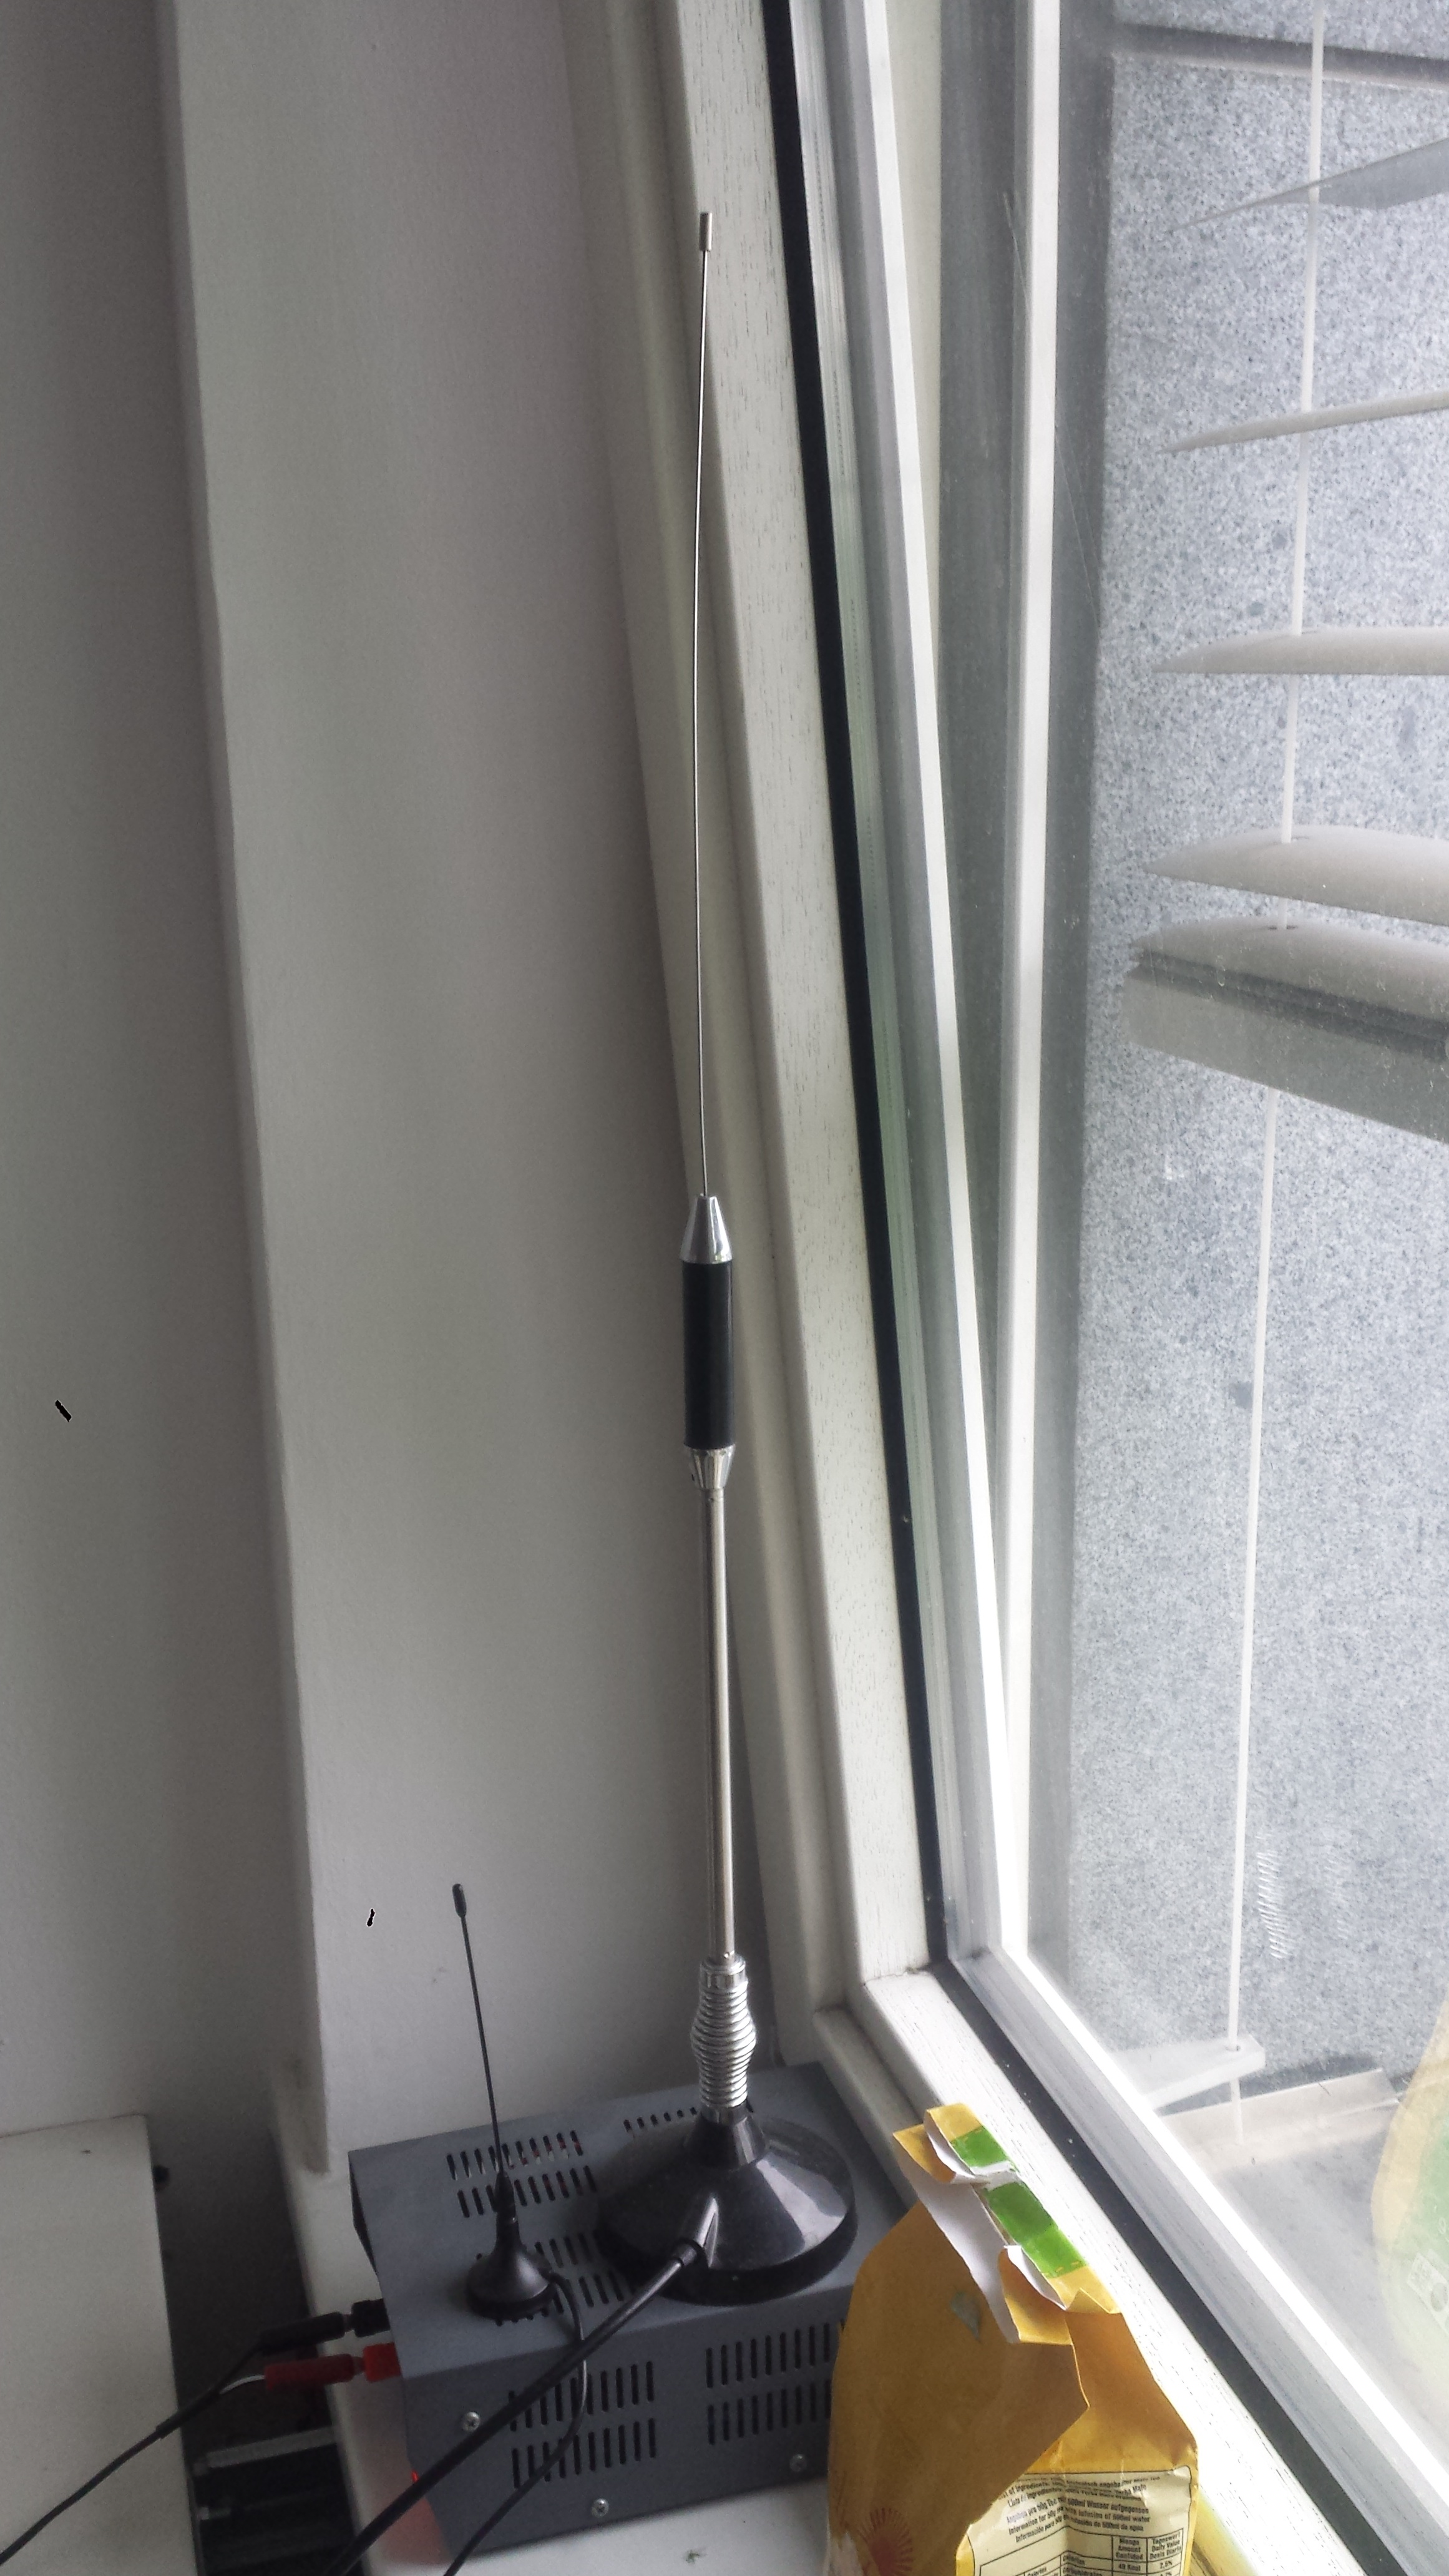
\includegraphics[width=0.8\textwidth]{a09/Verkurzte_10m_Antenne.jpg}\\
      \tiny Bild von DB4UM
    \end{center}
    \column{5cm} \large
    \begin{center}
      \begin{itemize}
        \item Mechanisch zu kurze Antennen können durch Induktivitäten verlängert werden.
        \item Zu lange Antennen können durch Kapazitäten elektrisch verkürtzt werden.
      \end{itemize}
    \end{center}
  \end{columns}
\end{frame}

\begin{frame}
  \frametitle{Realer Dipol}
  \begin{center}
    \begin{itemize}
      \item Da Antennendraht nicht unendlich dünn ist und immer Kapazitive Kopplung zum Erdboden besteht verstimmt sich die Antenne zu niedrigeren Frequenzen
      \item Beim Bau einer Realen Antenne mit Verkürzungsfaktoren so um $0.90-0.98$ rechnen.
    \end{itemize}
  \end{center}
\end{frame}

\section*{Richtdiagramm}

\begin{frame}
  \frametitle{Richtdiagramme erkennen}
  \begin{center}
    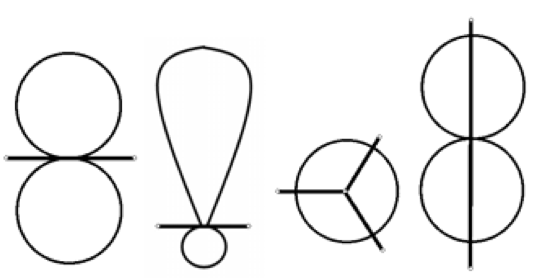
\includegraphics[width=0.95\textwidth]{a09/Abstrahl.png}
    \tiny \hyperlink{refs}{\cite{bna}} \\[1em] \large Welches Richtdiagramm ist welche Antenne?
  \end{center}
\end{frame}

\begin{frame}
  \frametitle{Halbwertsbreite}
  \begin{center}
    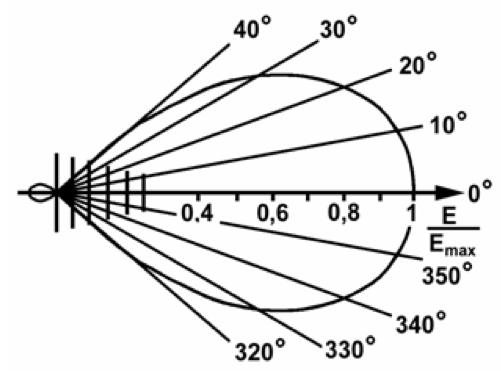
\includegraphics[width=0.7\textwidth]{a09/TH213.png}\\
    \tiny \hyperlink{refs}{\cite{bna}} TH213 \\[1em]
    \large Die Halbwertsbreite einer Antenne ist der Winkelbereich, innerhalb dem
    die Feldstärke auf nicht weniger als den 0,707-fachen Wert der maximalen Feldstärke absinkt.\\[1em] Wie viel Grad Öffnungswinkel hat dieser Richtstrahler?
  \end{center}
\end{frame}

\section*{Gewinn}

\begin{frame}
  \frametitle{Gewinn einer Antenne}
  \begin{center}
    \large Zum Messen Testaussendungen im Labor\\
    Vergleich oft mit Dipol\\
    \url{https://www.youtube.com/watch?v=gBqqp7rnZ64}\\[2em]
    $$g_D = 20 \cdot lg(\frac{P_{test}}{P_{dipol}}) = g_D[dBd]$$
    $$g_I = g_D + 2.5dB$$
  \end{center}
\end{frame}

\begin{frame}
  \frametitle{Vor-Rück Verhältnis, dBi, dBd}
  \begin{center}
    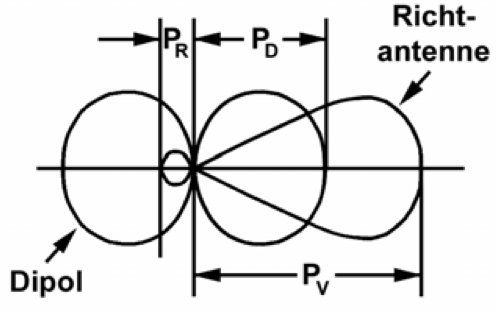
\includegraphics[width=0.8\textwidth]{a09/TH206.png}
    \tiny \hyperlink{refs}{\cite{bna}} \\[1em] \large Was ist das Vor-Rück Verhältnis, dBd und dBi ?
  \end{center}
\end{frame}


\section*{ERP, EIRP}

\begin{frame}
  \frametitle{ERP und EIRP}
  \begin{center}
    \Large $$P_{ERP} = g_{D} \cdot P_{sender}$$ \\
    $$P_{EIRP} = g_{I} \cdot P_{sender}$$ \\
    wobei $g_D + 2.15dB = g_I$
  \end{center}
\end{frame}

\section*{Antennentypen}

\begin{frame}
  \frametitle{Fuchskreis}
  \begin{center}
    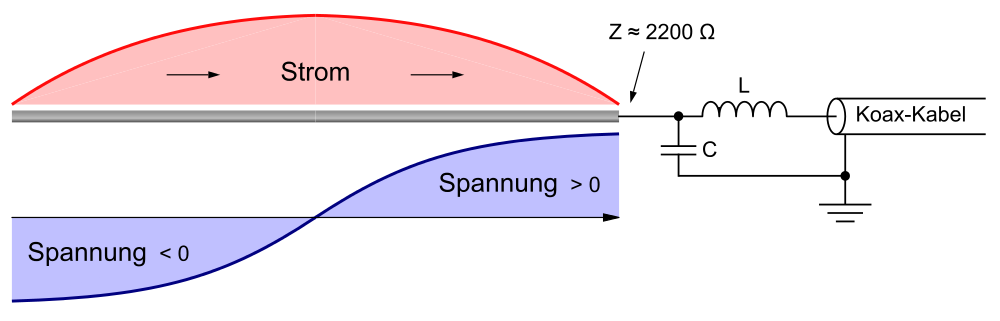
\includegraphics[width=1\textwidth]{a09/1000px-Endgespeiste_Antenne.png}
    \footnote{\tiny \url{https://commons.wikimedia.org/wiki/File:Endgespeiste_Antenne.svg}}
  \end{center}
\end{frame}

\section*{Multiband}

\begin{frame}
  \frametitle{Multibanddipol}
  \begin{center}
    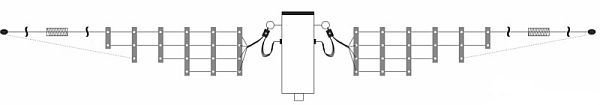
\includegraphics[width=0.9\textwidth]{a09/Multiband.jpg}
    \footnote{\tiny Antenne EA-1015204080 von EAntenna}
  \end{center}
\end{frame}

\begin{frame}
  \frametitle{G5RV}
  \begin{center}
    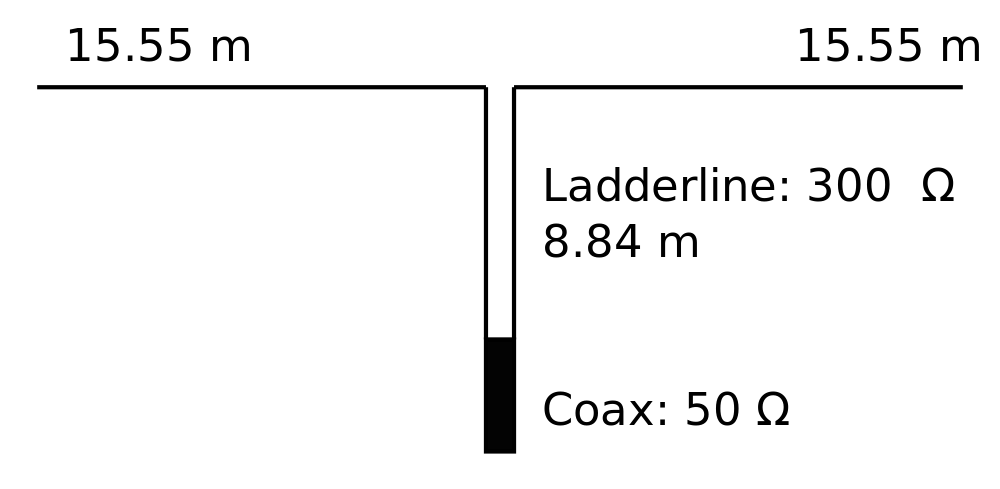
\includegraphics[width=0.9\textwidth]{a09/G5RV_Antenna.png}
    \footnote{\tiny \url{https://commons.wikimedia.org/wiki/File:G5RV_Antenna.svg}}
  \end{center}
\end{frame}

\begin{frame}
  \frametitle{W3DZZ}
  \begin{center}
    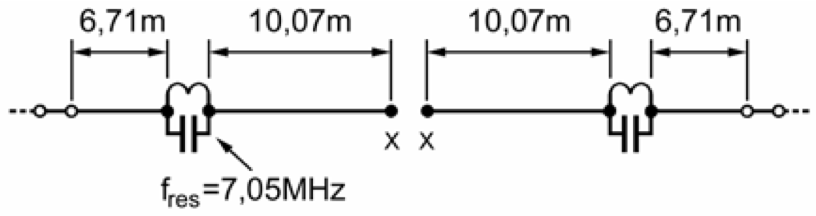
\includegraphics[width=1\textwidth]{a09/W3DZZ.png}
    \tiny \hyperlink{refs}{\cite{bna}} TH134
  \end{center}
\end{frame}

\begin{frame}
  \frametitle{Traps}
  \begin{center}
    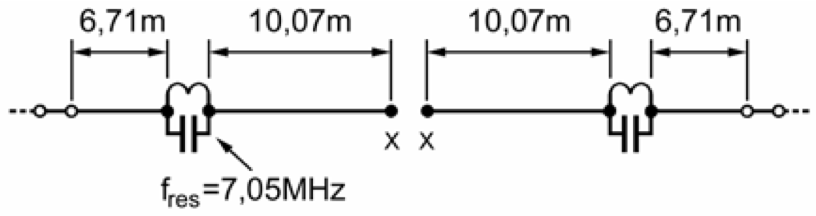
\includegraphics[width=1\textwidth]{a09/W3DZZ.png}
    \tiny \hyperlink{refs}{\cite{bna}} TH134 \\[1em] \large Wenn man diese Mehrband-Antenne auf 3,5 MHz erregt, dann wirken die LC-Resonanzkreise wie? \\[2em]
    Wenn man diese Mehrband-Antenne auf 7,05 MHz erregt, dann wirken die LC-Resonanzkreise wie?
  \end{center}
\end{frame}

\begin{frame}
  \frametitle{Windom}
  \begin{center}
    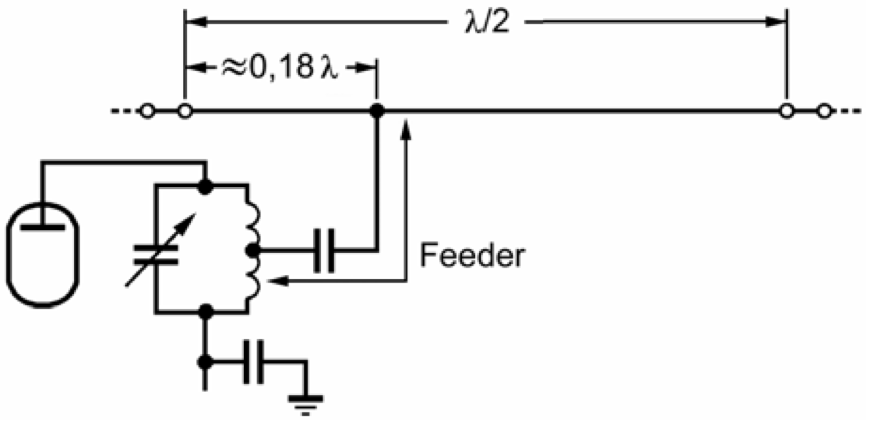
\includegraphics[width=1\textwidth]{a09/WINDOM_TH130.png}
    \tiny \hyperlink{refs}{\cite{bna}} TH134 \\[1em] \large Eindrehtspeiseleitung mit $500 \Omega$ \\[2em] Heutzutage kaum noch verwendet wegen zu vielen Umwelteinflüßen auf die Speiseleitung
  \end{center}
\end{frame}

\begin{frame}
  \frametitle{Yagi}
  \begin{center}
    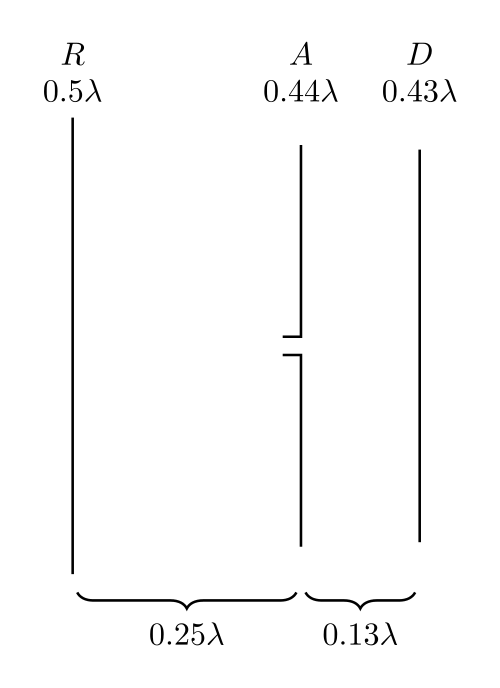
\includegraphics[width=0.5\textwidth]{a09/Yagi_3_element.png}
    \footnote{\tiny \url{https://commons.wikimedia.org/wiki/File:Yagi_3_element.svg}}
  \end{center}
\end{frame}

\begin{frame}
  \frametitle{Yagi - Richtung erkennen}
  \begin{center}
    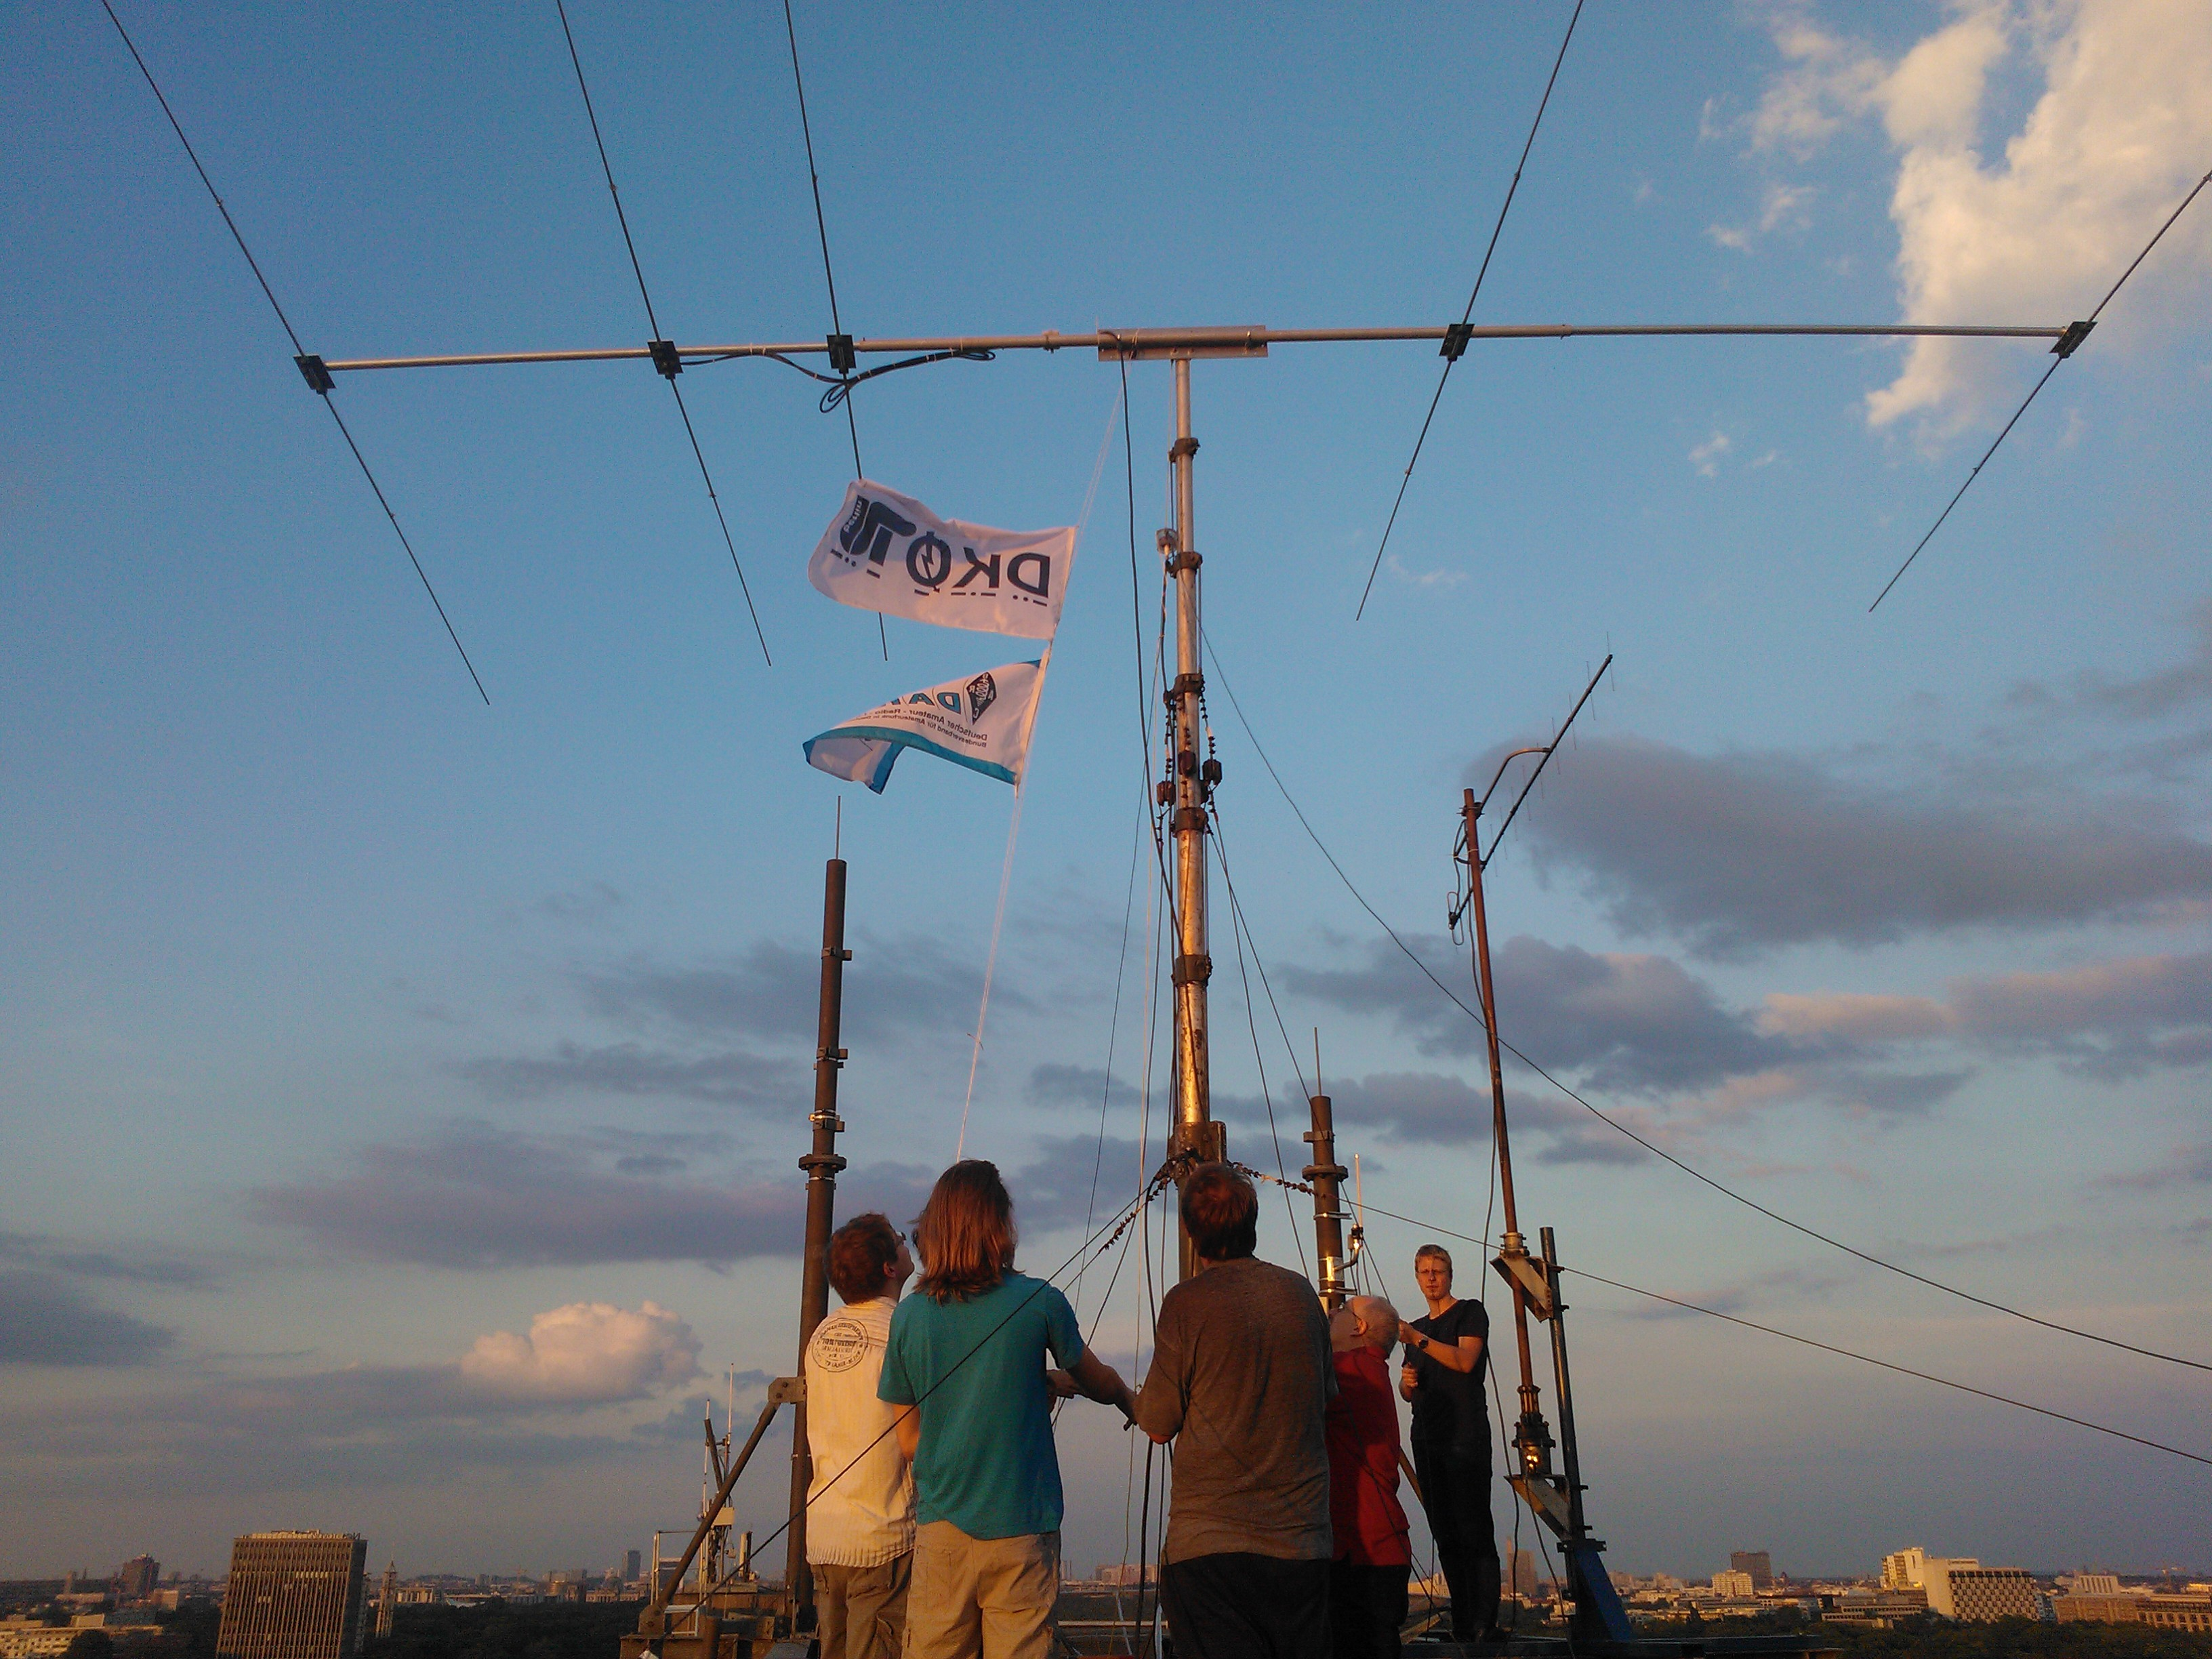
\includegraphics[width=.9\textwidth]{a09/yagi.jpg}
    \footnote{\tiny 10M Yagi bei DK0TU von DK9GD}
  \end{center}
\end{frame}

\begin{frame}
  \frametitle{Mehrband Beam}
  \begin{center} \large
    \begin{itemize}
      \item Kreuzung aus dem Dipol mit Traps und der Yagi-Antenne
      \item Bereich mit guter Resonanz ist schmaler, aber Antenne kürzer.
    \end{itemize}
  \end{center}
\end{frame}

\section*{Vertikalantennen}

\begin{frame}
  \frametitle{Groundplane oder Marconi-Antenne}
  \begin{center}
    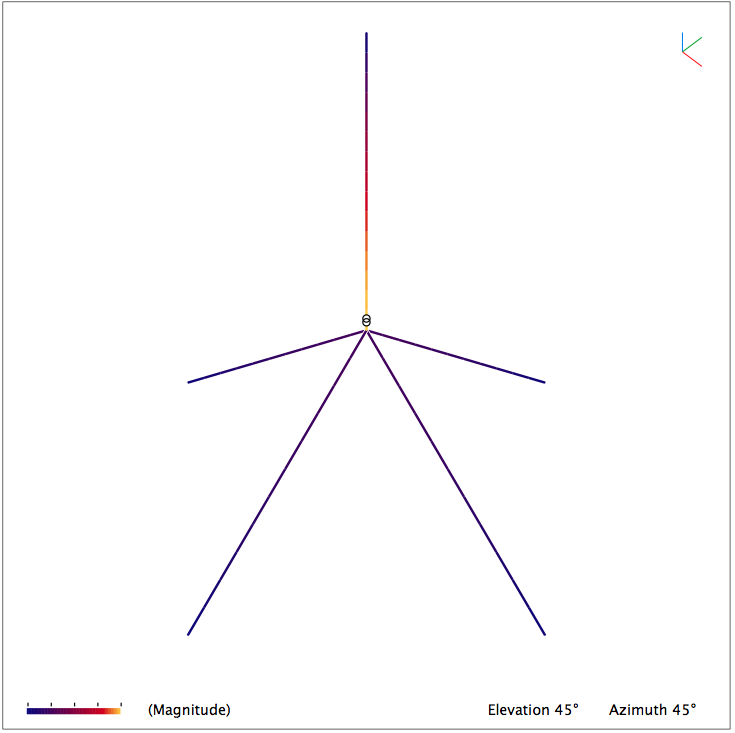
\includegraphics[width=0.7\textwidth]{a09/GP-DB4UM.png}
    \footnote{\tiny DB4UM mit cocoaNec 2.0}
  \end{center}
\end{frame}

\begin{frame}
  \frametitle{Dipol mit Ground}
  \begin{center}
    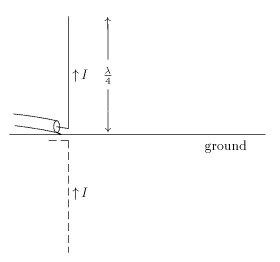
\includegraphics[width=0.7\textwidth]{a09/A6-3EN.jpg}
    \tiny \hyperlink{refs}{\cite{wm}} \\[2em] \large
    Der Boden bewirkt wie eine Spiegelung elektrisch invertierte des Strahlers
  \end{center}
\end{frame}

\begin{frame}
  \frametitle{Spezille Antennen}
  \begin{center}
    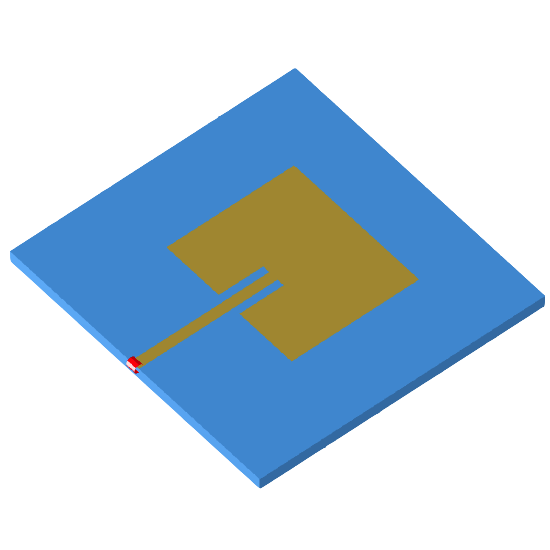
\includegraphics[width=1\textwidth]{a09/patch.png}

  \end{center}
\end{frame}

\begin{frame}
  \frametitle{Magnetic Loop}
  \begin{center}
    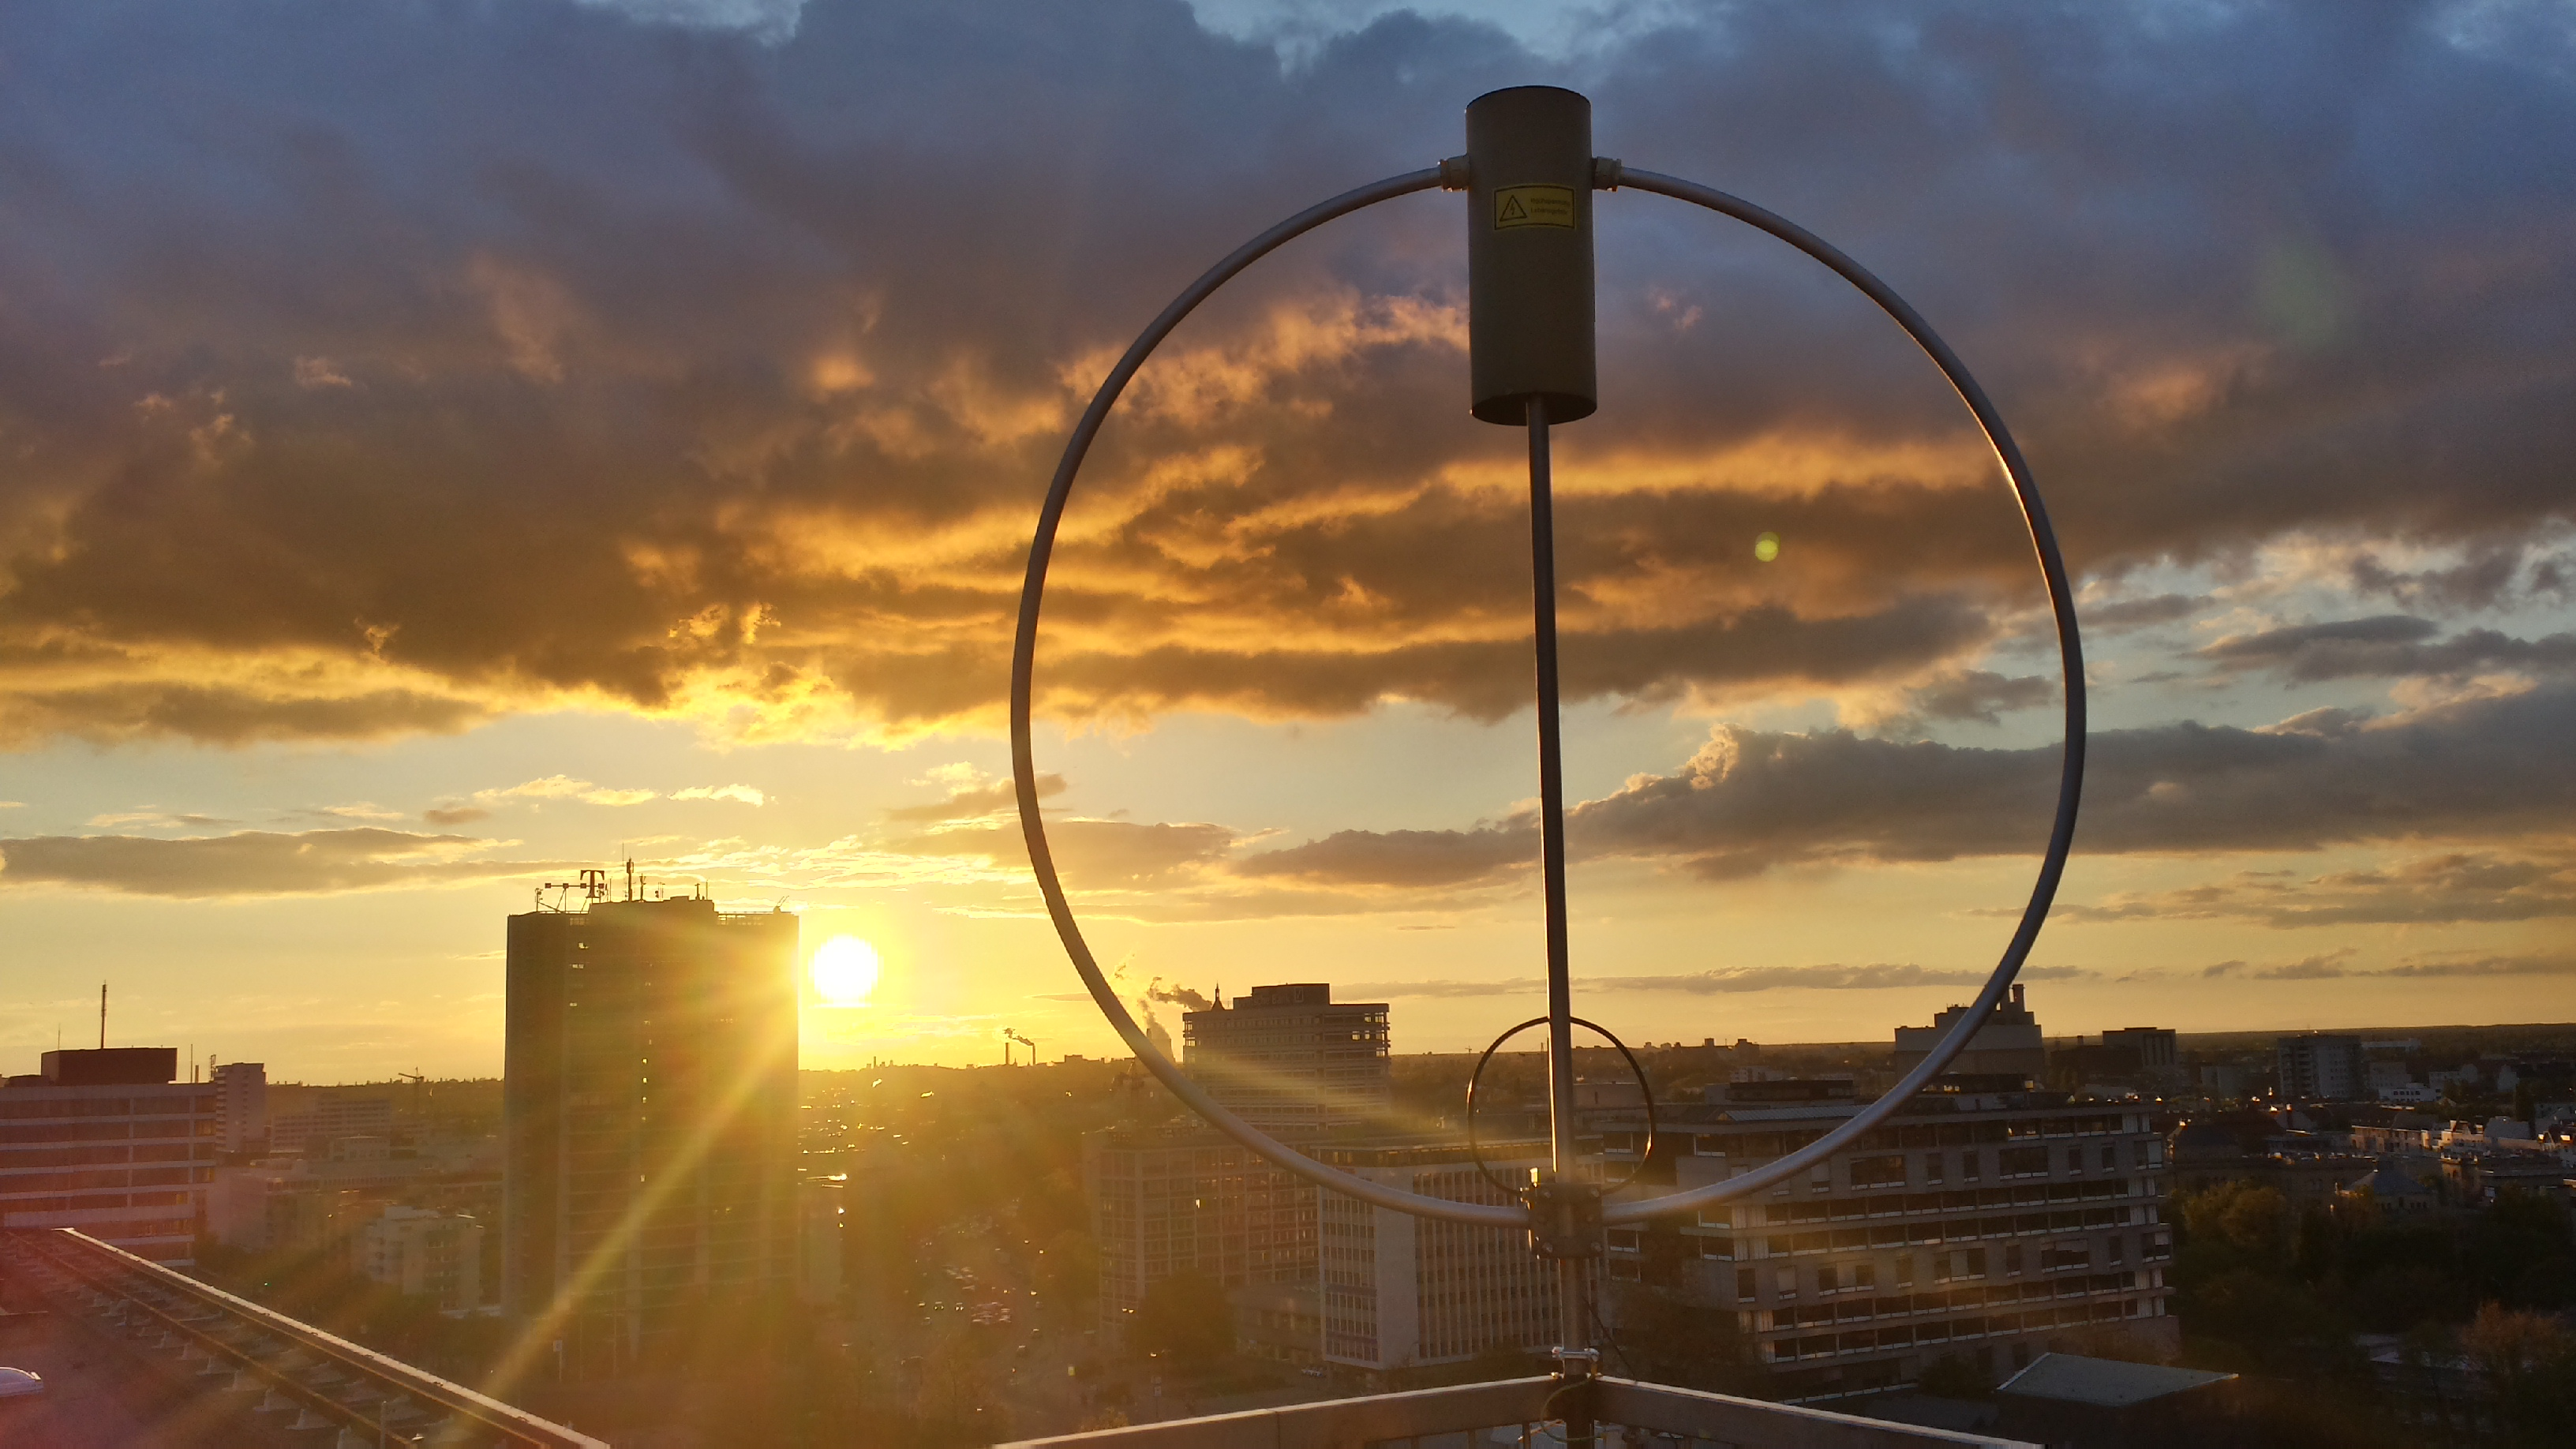
\includegraphics[width=1\textwidth]{a09/Magloop.jpg}
    \footnote{\tiny Magloop bei DK0TU von DB4UM}
  \end{center}
\end{frame}

\begin{frame}
  \frametitle{Spiegel Antenne}
  \begin{center}
    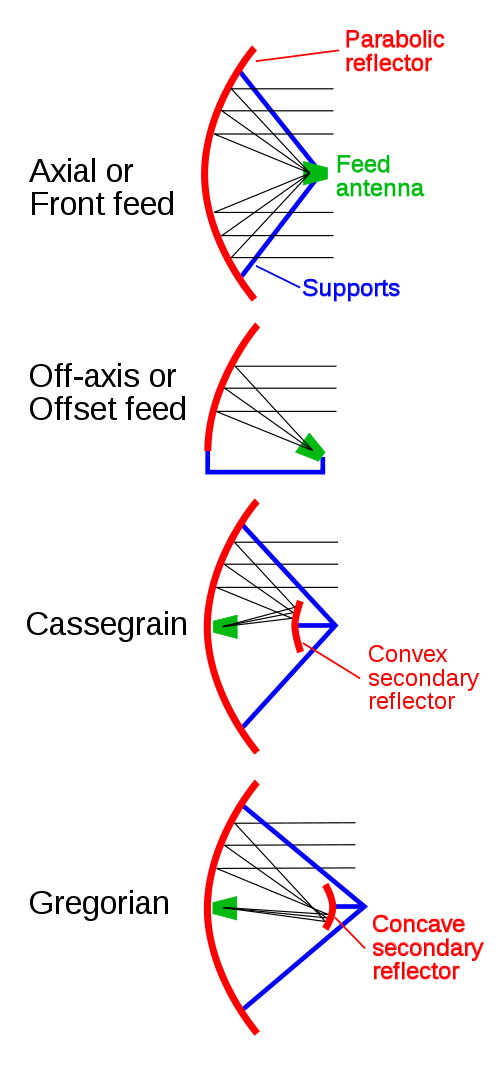
\includegraphics[width=0.4\textwidth]{a09/Parabolic_antenna_types.png}
    \tiny \hyperlink{refs}{\cite{wm}}
  \end{center}
\end{frame}


\begin{frame}
  \frametitle{Helix Antenne}
  \begin{center}
    \includegraphics[width=0.6\textwidth]{a09/Traqueur_acquisition.JPG}
    \tiny \hyperlink{refs}{\cite{wm}}
  \end{center}
\end{frame}

\begin{frame}
  \frametitle{Portabelfunken in Berlin}
  \begin{columns}[c]
    \column[c]{5cm}
    \begin{center}
      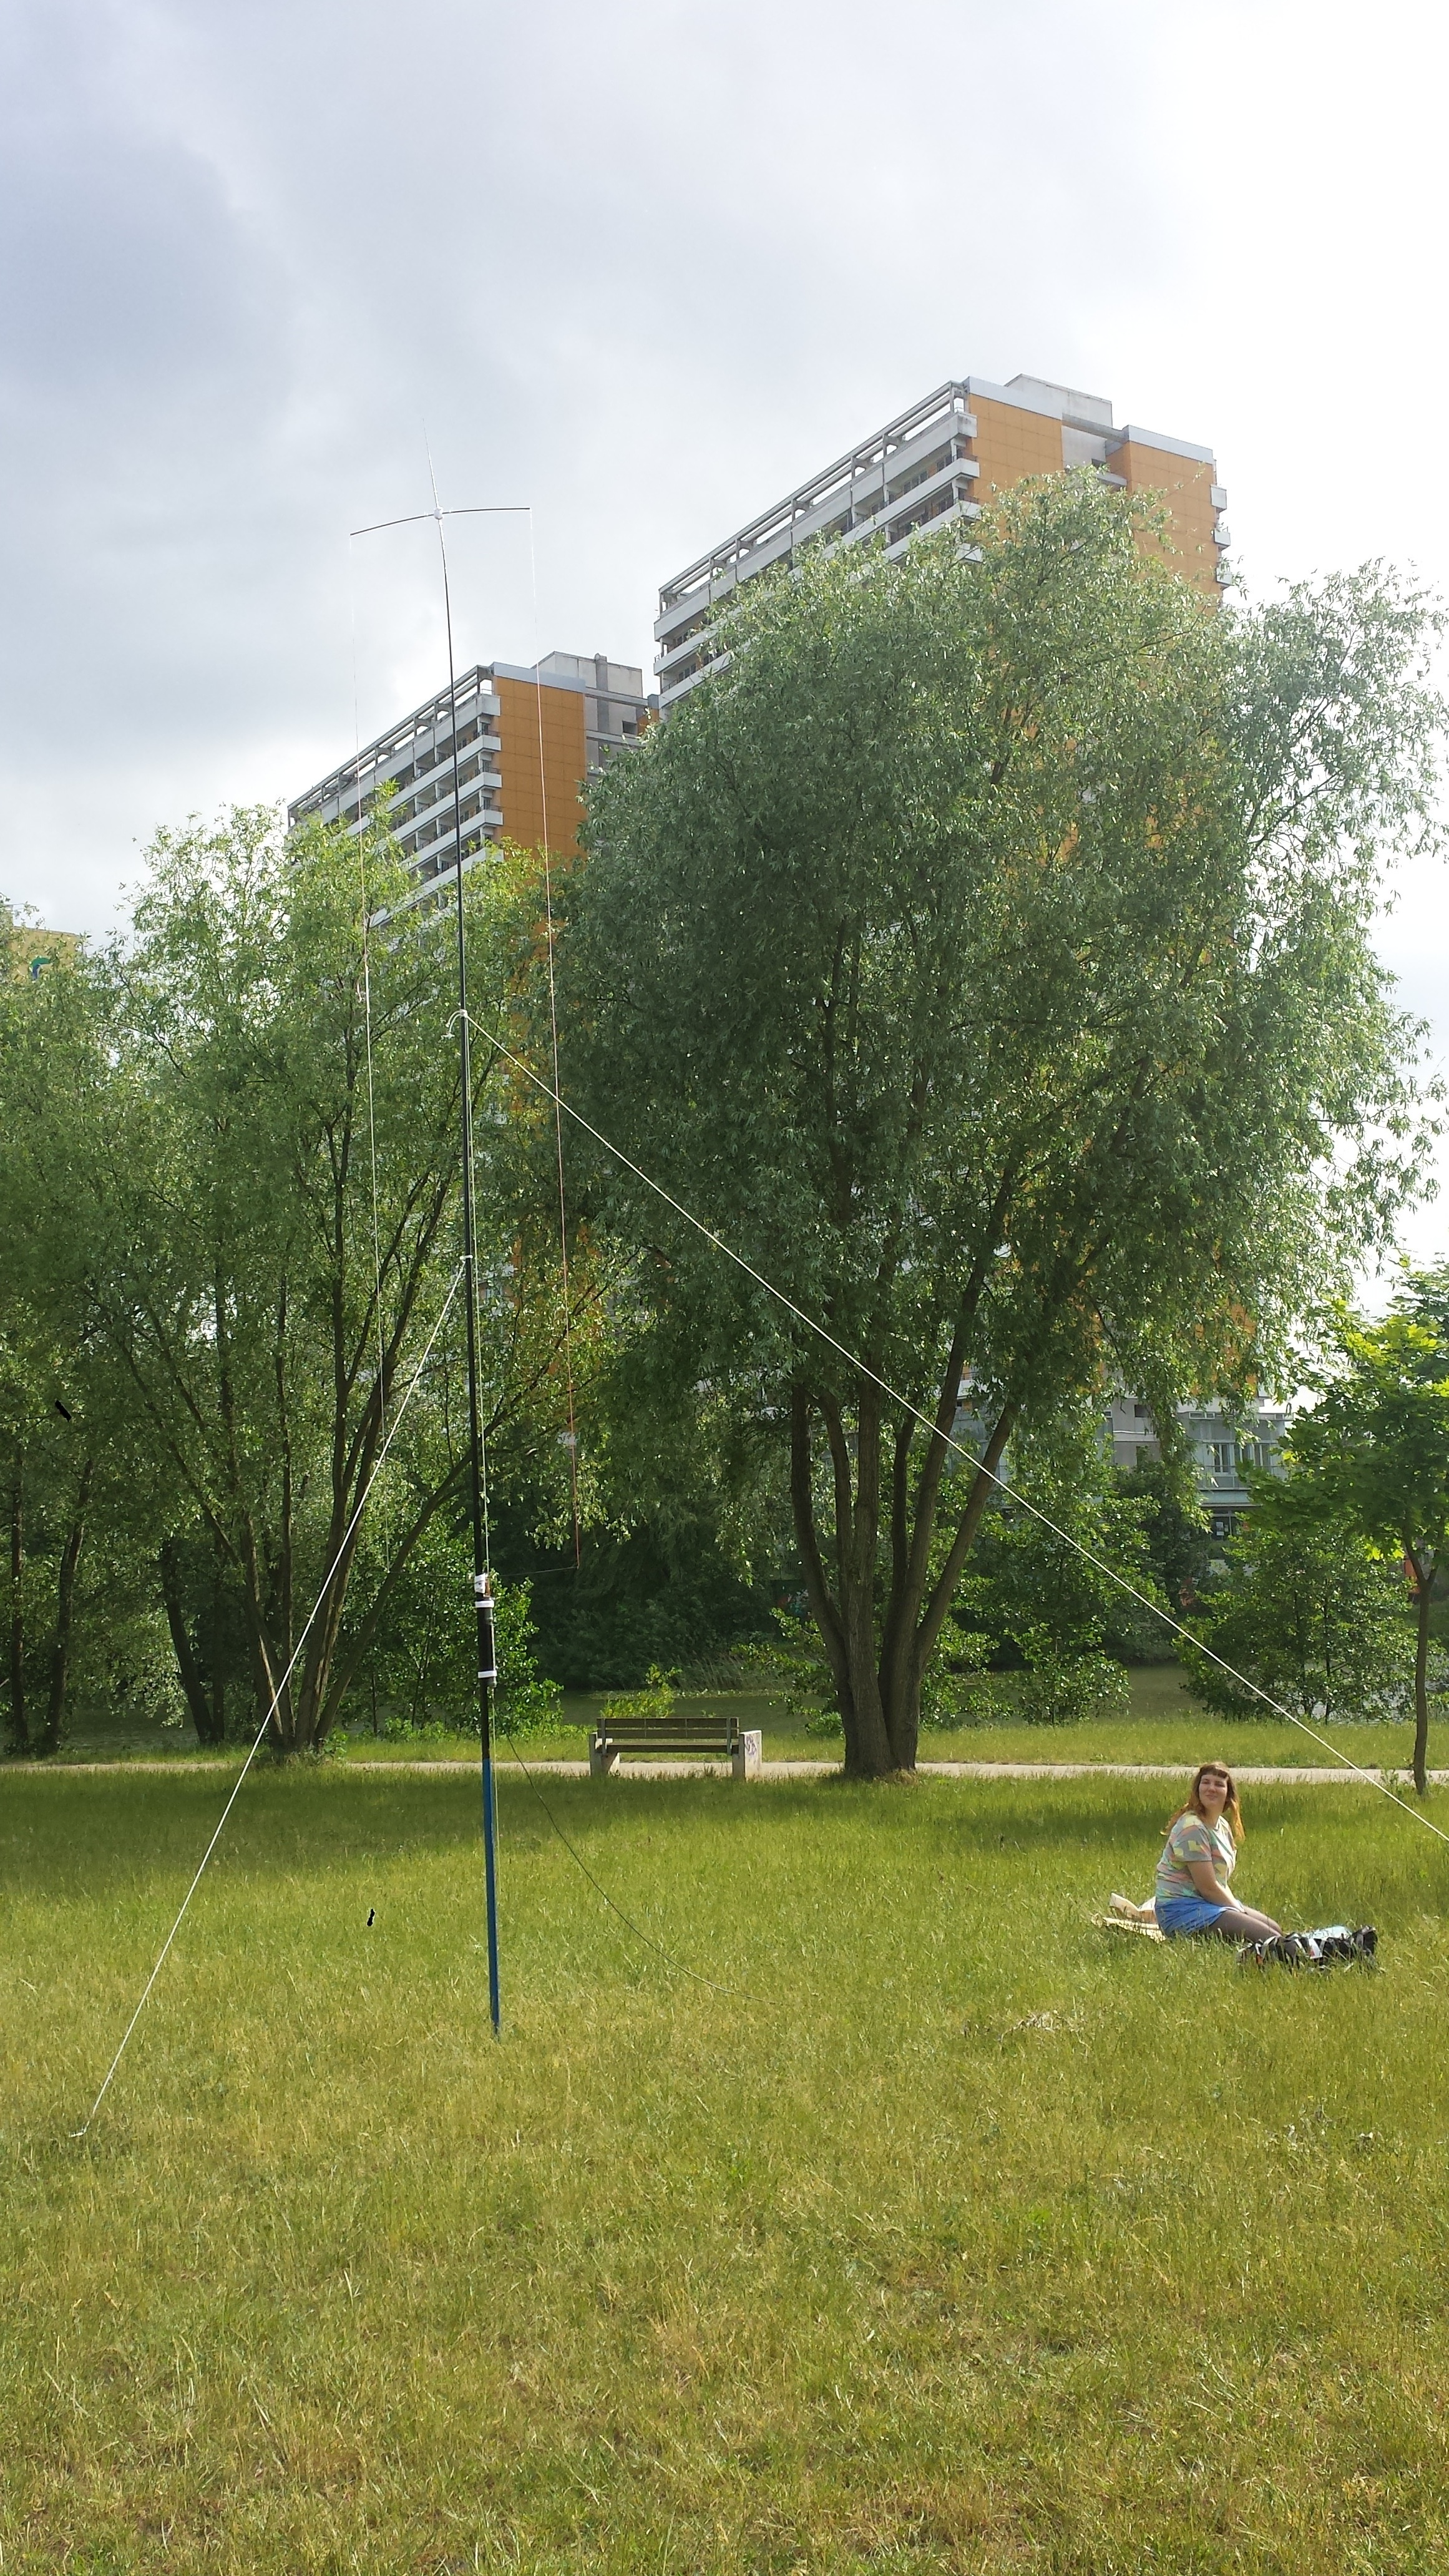
\includegraphics[width=0.82\textwidth]{a09/db4um_dm1ri_portabel.jpg}\\
      \tiny C-Pole im Springpfuhl Bild: DB4UM
    \end{center}
    \column{5cm} \large
    \begin{center}
      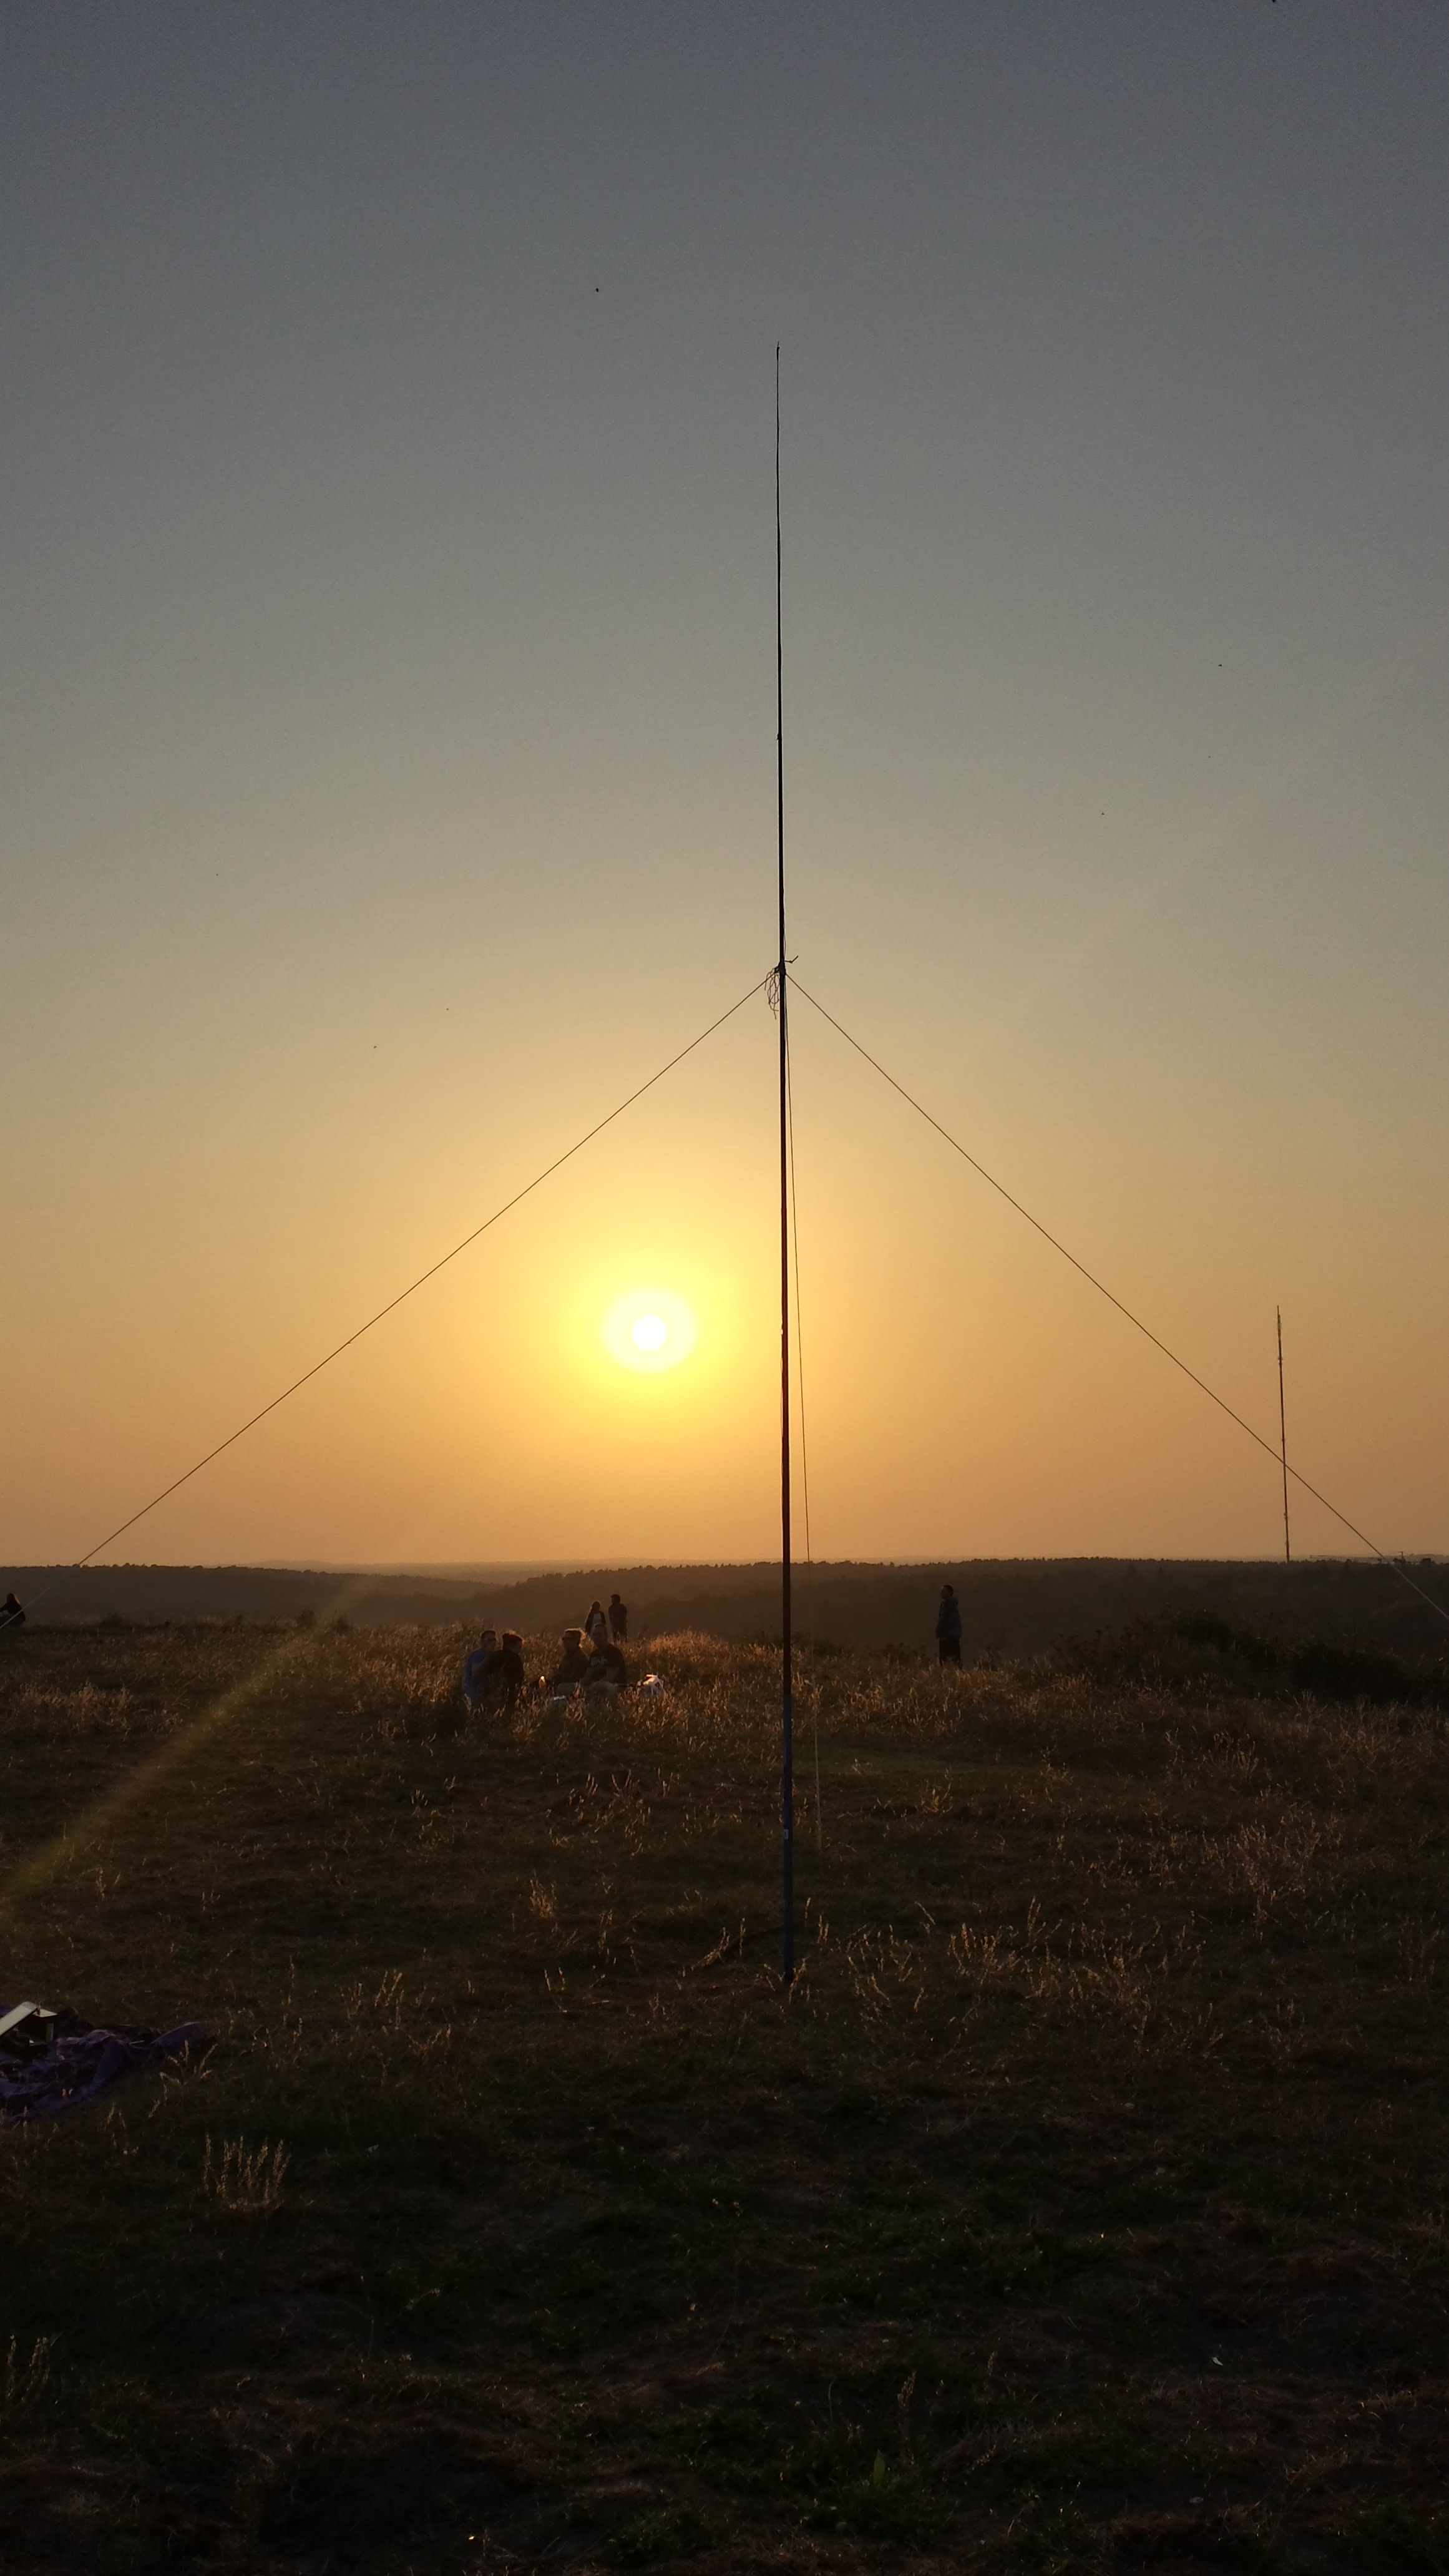
\includegraphics[width=0.82\textwidth]{a09/db4um_Drachenberg.jpg}\\
      \tiny Groundplane auf dem Drachenberg Bild: DB4UM
    \end{center}
  \end{columns}
\end{frame}

\begin{frame}
  \frametitle{Kurzwellensender Nauen}
  \begin{center}
    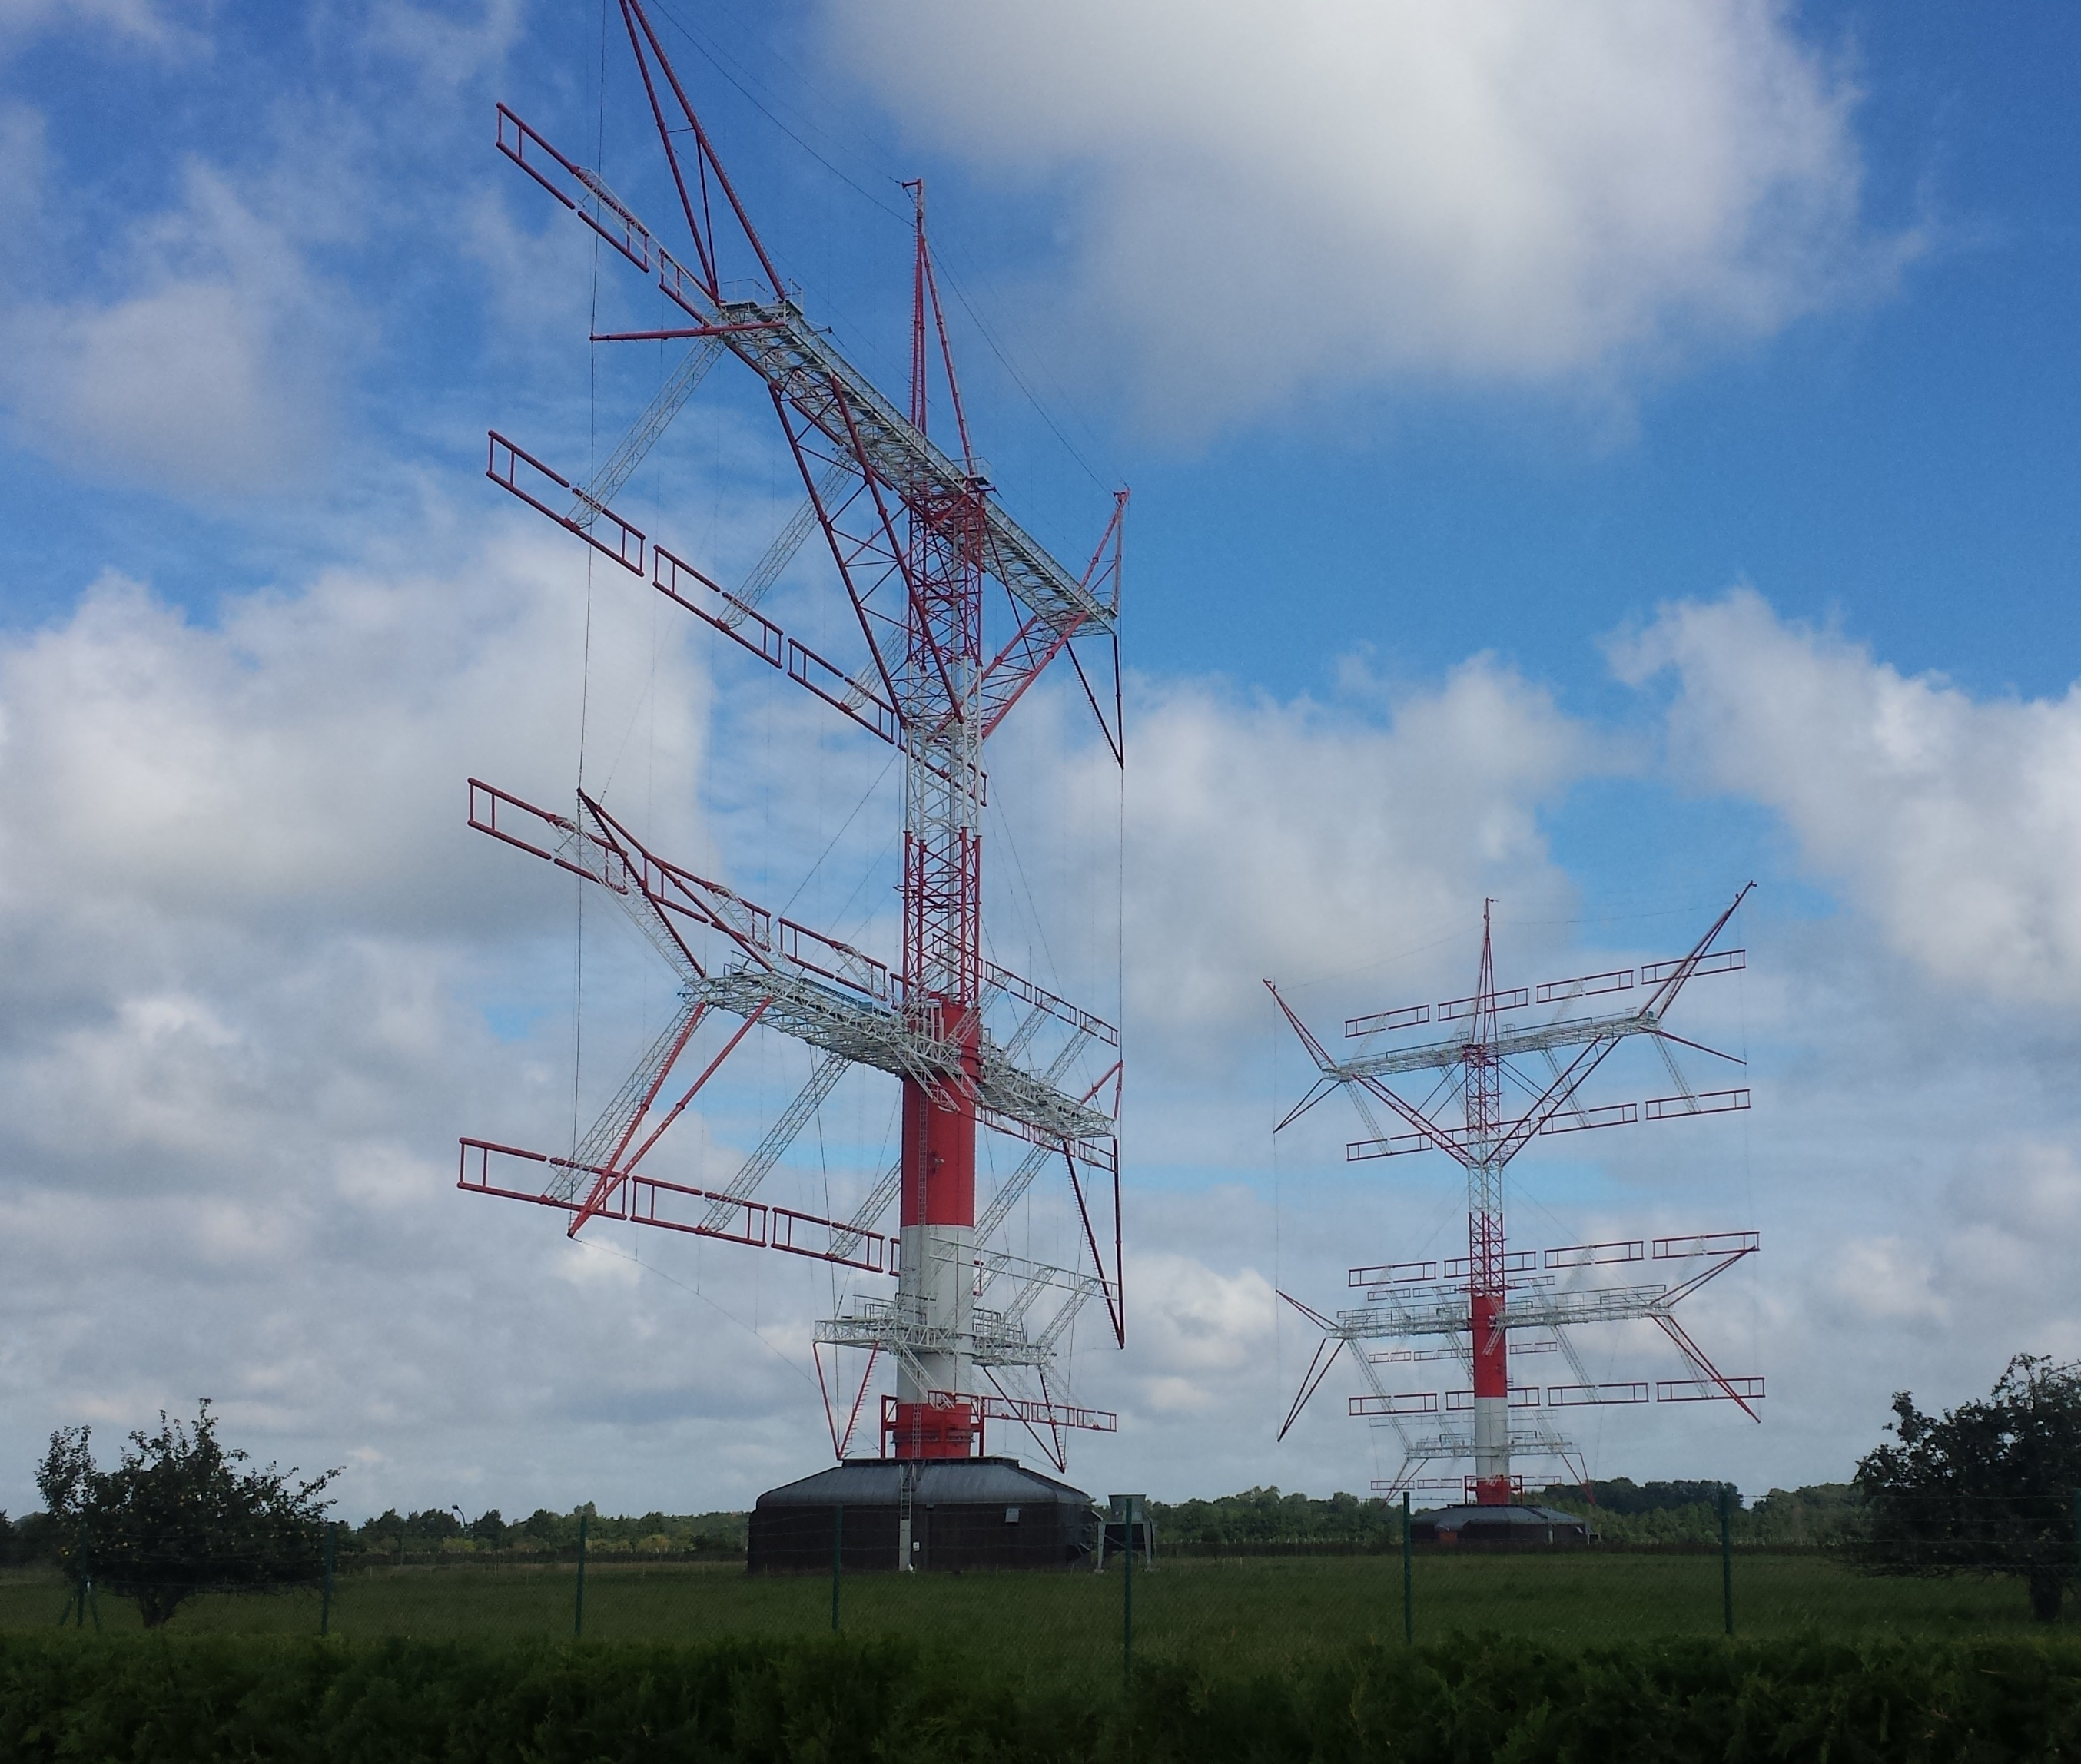
\includegraphics[width=0.93\textwidth]{a09/Nauen_Dipolarray.jpg}\\
    \tiny Kurzwellensenderantennen in Nauen Bild: DB4UM
  \end{center}
\end{frame}



\renewcommand{\refname}{Referenzen}

\hypertarget{refs}{}
\textcolor{white}{} \\ %\vspace{} geht nicht
\Large Referenzen/Links
\footnotesize

\begin{thebibliography}{}
  \bibitem{darc}  DARC Online-Lehrgang Lektion A08:
    \url{https://www.darc.de/der-club/referate/ajw/lehrgang-ta/a09/}
  \bibitem{wm}  Wikimedia:
    \url{https://upload.wikimedia.org/wikipedia/commons/3/32/Traqueur_acquisition.JPG}
    \url{https://commons.wikimedia.org/wiki/File:Felder_um_Dipol.jpg}
    \url{https://commons.wikimedia.org/wiki/File:Lineare_antennen.svg}
    \url{https://commons.wikimedia.org/wiki/File:Lineare_antennen.svg}
    \url{https://commons.wikimedia.org/wiki/File:Dipole_Antenna.svg}
    \url{https://commons.wikimedia.org/wiki/File:G5RV_Antenna.svg}
    \url{https://commons.wikimedia.org/wiki/File:Endgespeiste_Antenne.svg}
    \url{https://commons.wikimedia.org/wiki/File:Yagi_3_element.svg}
    \url{https://commons.wikimedia.org/wiki/File:FWHM.svg}
    \url{https://commons.wikimedia.org/wiki/File:Parabolic_antenna_types2.svg}
    \url{https://commons.wikimedia.org/wiki/File:A6-3EN.jpg}
    \url{}
  \bibitem{beam}  Beamkarten Generator von NS6T:
    \url{http://ns6t.net/azimuth/azimuth.html}
  \bibitem{wp}    Wikipedia - Die freie Enzyklopädie:
    \url{https://de.wikipedia.org/wiki/Dipolantenne}
  \bibitem{bna}   Fragenkatalog Bundesnetzargentur Technik Klasse A:
    \url{https://www.bundesnetzagentur.de/SharedDocs/Downloads/DE/Sachgebiete/Telekommunikation/Unternehmen_Institutionen/Frequenzen/Amateurfunk/Fragenkatalog/TechnikFragenkatalogKlasseAf252rId9014pdf.pdf?__blob=publicationFile&v=3}
\end{thebibliography}

% Hier könnte noch eine Kontaktfolie stehen

\end{document}

